\documentclass{article}

% if you need to pass options to natbib, use, e.g.:
% \PassOptionsToPackage{numbers, compress}{natbib}
% before loading nips_2018

% ready for submission
\usepackage{nips_2018}
\usepackage{enumitem}
% to compile a preprint version, e.g., for submission to arXiv, add
% add the [preprint] option:
%\usepackage[preprint]{nips_2018}

% to compile a camera-ready version, add the [final] option, e.g.:
% \usepackage[final]{nips_2018}

% to avoid loading the natbib package, add option nonatbib:
% \usepackage[nonatbib]{nips_2018}

\usepackage[T1]{fontenc}    % use 8-bit T1 fonts
\usepackage{hyperref}       % hyperlinks
\usepackage{url}            % simple URL typesetting
\usepackage{booktabs}       % professional-quality tables
\usepackage{amsfonts}       % blackboard math symbols
\usepackage{nicefrac}       % compact symbols for 1/2, etc.
\usepackage{wrapfig}
\usepackage{picins}

\usepackage[backgroundcolor = White,textwidth=2cm]{todonotes}
%\usepackage[disable,backgroundcolor = White,textwidth=\marginparwidth]{todonotes}
\newcommand{\todom}[2][]{\todo[color=orange!25,size=\small,#1]{G: #2}}
\newcommand{\todox}[2][]{\todo[color=purple!25,size=\small,#1]{K: #2}}
\newcommand{\todor}[2][]{\todo[color=blue!25,size=\small,#1]{R: #2}}
\setlength{\marginparwidth}{0.8in}

\usepackage[margin=1in]{geometry}

% Set the typeface to Times Roman
\usepackage{times}

\usepackage{algorithm,algorithmic}
\newcommand{\theHalgorithm}{\arabic{algorithm}}

\usepackage{microtype}
\usepackage{graphicx}
\usepackage{subfigure}
\usepackage{booktabs} % for professional tables

\usepackage{natbib}

\usepackage{amssymb} %maths
\usepackage{amsmath} %maths
\usepackage{amsthm}
\usepackage{hyperref}
\usepackage[utf8]{inputenc} %useful to type directly diacritic characters
\usepackage[capitalize]{cleveref}
\crefname{prop}{Proposition}{Propositions}
\crefname{thm}{Theorem}{Theorems}
\crefname{lem}{Lemma}{Lemmas}
\crefname{algorithm}{Algorithm}{Algorithms}

\def\rva{{\mathbf{a}}}
\def\rvo{{\mathbf{o}}}
\def\rvr{{\mathbf{r}}}
\def\rvs{{\mathbf{s}}}
\def\rvu{{\mathbf{u}}}
\def\rvw{{\mathbf{w}}}
\def\rvx{{\mathbf{x}}}
\def\rvg{{\mathbf{g}}}
\def\rvo{{\mathbf{o}}}
\def\rvone{{\mathbf{1}}}
\def\rvzero{{\mathbf{0}}}
\def\rvtilder{{\tilde{\mathbf{r}}}}
\def\rvhat{{\hat{\mathbf{r}}}}

\def\rvp{{\mathbf{p}}}

\def\pr{{\text{Pr}}}
\def\r{{\text{R}}}

\def\ucb{{\text{U}}}
\def\lcb{{\text{L}}}

\newtheorem{thm}{Theorem}
\newtheorem{lem}{Lemma}
\newtheorem{defi}{Definition}
\newtheorem{prop}{Proposition}
\newtheorem{remk}{Remark}

\def\rvpi{{\boldsymbol{\pi}}}

\def\rmA{{\mathbf{A}}}
\def\rmD{{\mathbf{D}}}
\def\rmH{{\mathbf{H}}}
\def\rmI{{\mathbf{I}}}
\def\rmW{{\mathbf{W}}}
\def\rmX{{\mathbf{X}}}

\def\sE{{\mathbb{E}}}
\def\sR{{\mathbb{R}}}
\def\sI{{\mathbb{I}}}
\def\sP{{\mathbb{P}}}

\def\gN{{\mathcal{N}}}
\def\gE{{\mathcal{E}}}
\def\gU{{\mathcal{U}}}

\DeclareMathOperator*{\argmax}{arg\,max}
\DeclareMathOperator*{\argmin}{arg\,min}
\DeclareMathOperator*{\probability}{Pr}
\DeclareMathOperator*{\expectation}{\sE}

\renewcommand{\algorithmicrequire}{\textbf{Input:}}
\renewcommand{\algorithmicensure}{\textbf{Output:}}

\title{On Provable Policy Gradient Methods and Optimal Stochastic Bandit Algorithms with Neural Networks}

% The \author macro works with any number of authors. There are two
% commands used to separate the names and addresses of multiple
% authors: \And and \AND.
%
% Using \And between authors leaves it to LaTeX to determine where to
% break the lines. Using \AND forces a line break at that point. So,
% if LaTeX puts 3 of 4 authors names on the first line, and the last
% on the second line, try using \AND instead of \And before the third
% author name.

\author{
  David S.~Hippocampus\thanks{Use footnote for providing further
    information about author (webpage, alternative
    address)---\emph{not} for acknowledging funding agencies.} \\
  Department of Computer Science\\
  Cranberry-Lemon University\\
  Pittsburgh, PA 15213 \\
  \texttt{hippo@cs.cranberry-lemon.edu} \\
  %% examples of more authors
  %% \And
  %% Coauthor \\
  %% Affiliation \\
  %% Address \\
  %% \texttt{email} \\
  %% \AND
  %% Coauthor \\
  %% Affiliation \\
  %% Address \\
  %% \texttt{email} \\
  %% \And
  %% Coauthor \\
  %% Affiliation \\
  %% Address \\
  %% \texttt{email} \\
  %% \And
  %% Coauthor \\
  %% Affiliation \\
  %% Address \\
  %% \texttt{email} \\
}

\begin{document}
% \nipsfinalcopy is no longer used

\maketitle

\begin{abstract}
In this paper, we propose a deep reinforcement learning algorithm which achieves nearly optimal finite time regret in the stochastic bandit setting. In our method, the agent maintains its action selection strategy in a parametric fashion. After enough exploration, a neural network is trained to minimized the empirical value related objectives using gradient updates. The policy is obtained from the exponential weight of learned logits. While our method is unlike standard bandit algorithms which directly utilize statistics from samples, we show that its finite time regret is nearly optimal up to log and constant factor. The results can be generalized to episodic MDPs and the state dependent bandit cases.
\end{abstract}

\section{Introduction}
\label{introduction}

Deep Reinforcement Learning (DRL) has recently achieved great successes, including games \citep{silver2016masteringA,silver2017masteringB,moravvcik2017deepstack,mnih2015human}, robotics \citep{lillicrap2015continuous,levine2016end}, just name a few. However, comparing with its brilliant achievements, the theoretical understanding of the mechanism behind DRL methods is not enough to explain its practical performance. 

DRL combines techniques in Deep Learning (DL) and Reinforcement Learning (RL) fields, to understand DRL, we need findings from both the DL and the RL sides.

On the RL side, it is well studied that under the bandit settings, and the tabular cases of the Markov decision process (MDP) setting, a number of algorithms enjoy favorable theoretical guarantees \citep{bubeck2012regret,sutton2018reinforcement}. In particular, either the optimal policies can be learned asymptotically, or within finite time, sublinear regret can be obtained. However, once it goes beyond the tabular cases, the theoretical results become much weaker. For example, Gradient Temporal Difference (GTD) with (non-)linear function approximations can only converge to the fixed points of projected Bellman operators \citep{sutton2009fast,sutton2009convergent,bhatnagar2009convergent}. While the performance of the fixed point policies can be arbitrarily bad without any further assumptions on the function approximations.

On the DL side, the empirical achievements are also much more advanced than the  theoretical results \citep{goodfellow2016deep}. However, there are still progresses in the expressiveness, optimization, and generalization aspects of DL theory. In particular, very recently, it has been discovered that, in supervised learning (regression and classification) settings, the training loss can be globally optimized (in linear convergence rate for $\ell_2$ loss in regression, and in constant time for classification) by gradient descent (GD) and stochastic gradient descent (SGD) method, given that the number of parameters in hidden layer is quite large, i.e., overparameterization. With some additional structured data distribution assumptions, the convergent training loss can be generalized to testing loss, making the neural network have provable generalization ability. 

To combine progresses in the DL and RL fields, we consider two main diferences between RL and supervised learning: (a) unlike the supervised learning settings, there are no true labels when learning RL agents; (b) to learn good agents, enough exploration is necessary.

In this paper, based on the recent progresses in overparameterized neural network optimization, we make one step forward to theoretically understanding DRL. In particular, we make the following contributions.
\begin{itemize}
    \item We prove that in bandit setting, with enough exploration, the widely-used policy gradient method, with policy net represented by a overparameterized two layer neural network (NN), achieves $O\left( \sqrt{T} \right)$ regret.
    \item We show that in episodic MDP setting, with the same exploration strategy and policy net as above, policy gradient method achieves $O\left( \sqrt{T} \right)$ regret.
    \item In many state dependent bandit and MDP settings, similar results also hold.
\end{itemize}

We would like to point that the above results can be generalized to policy net represented by multi-layered neural networks. Assuming a two layer NN policy is just for simplicity and conciseness. We provide the generalization to multi-layered NN in the appendix for completeness.

To our knowledge, our finding is the first convergence result for popular RL methods (here, policy gradient) with non-linear NN function approximations, which provides theoretical support for DRL methods. Our result is just beginning of understanding many other DRL methods (such as DQN \cite{mnih2015human}, A3C \citep{mnih2016asynchronous}, and PCL \citep{nachum2017bridging}), with more practical NN function approximations (e.g., less overparameterized), using many other policy optimization techniques (such as mirror descent, and relative entropy policy search).

The rest of the paper is organized as follows. Some proofs are deferred to appendix due to space limit.

\subsection{Notations}

Bold letters refer to vectors, and non-bold letters refer to scalars. For example, $u_{i,r} \in \sR$ is the $r$th component of vector $\rvu_i \in \sR^m$. $n$ is the total number of states, while $m$ is the total number of nodes in each hidden layer. $h$ is the total number of actions can be taken at each state. $\rvone$ means all-one vector, and $\rmI$ refers to identity matrix, with dimensions depends on the contexts.

Denote $[n] \triangleq \left\{ 1,2, \dots, n \right\}$. $\rvs_i \in \sR^d$, $i \in [n]$ refers to a state. $\rvw_r \in \sR^d$, $r \in [m]$ is a weight vector in the first hidden layer. $\rmW^\top \triangleq \left[ \rvw_1, \rvw_2, \dots, \rvw_m \right] \in \sR^{d \times m}$ is the weight matrix of the first hidden layer. $u_{i,r} \triangleq \rvw_r^\top \rvs_i$ is the $r$th node value of the first hidden layer. $\rva_k \in \sR^m$, $k \in [h]$ is a weight vector in the second hidden layer. In the paper, after the random initialization $\rva_k \sim \gU\left\{-1, +1\right\}$, $\rva_k$ will be fixed. This assumption is common in literature \citep{li2018learning,du2018gradientA,du2018gradientB,allen2018convergenceA,allen2018convergenceB}, and has been empirically verified that has no impact on the performance of trained neural networks \citep{hoffer2018fix}. Other initialization like $\rva_k \sim \gN(0, \rmI)$ also works. $\rmA^\top \triangleq \left[ \rva_1, \rva_2, \dots, \rva_h \right] \in \sR^{m \times h}$ is the weight matrix of the second hidden layer. $o_{i,k} \triangleq \sum\limits_{r=1}^{m}{a_{k,r} \cdot \sigma\left( u_{i,r} \right)}$ is the logit of the $k$th action for state $\rvs_i$, where $\sigma(\cdot) \triangleq \max\left\{ \cdot, 0 \right\}$ is the ReLU activation function. $\pi_{i,k} \triangleq f\left( o_{i,k} \right) \triangleq \frac{\exp\left\{ o_{i,k} \right\}}{\sum\limits_{k^\prime = 1}^{h}{\exp\left\{ o_{i,k^\prime} \right\}}}$ is the probability of choosing action $k$ at state $\rvs_i$, where $f(\cdot)$ is the softmax function. $\rvr_i \in \sR^h$ is the true reward vector at state $\rvs_i$. $\r_i^{\max} \triangleq \max\limits_{k \in [h]}\left\{ r_{i,k} \right\}$ is the maximum reward at state $\rvs_i$. $\rvtilder_i \triangleq \r_i^{\max} \cdot \rvone - \rvr_i$ is the true loss vector at state $\rvs_i$. Given stochastic policies $\rvpi \triangleq \left[ \rvpi_1, \rvpi_2, \dots, \rvpi_n \right] \in \sR^{h \times n}$, the expected loss is defined as,
\begin{equation}
\label{eq:expected_loss}
\begin{split}
    \ell \triangleq \frac{1}{n} \cdot \sum\limits_{i=1}^{n}{ \left( \r_i^{\max} - \rvpi_i^\top \rvr_i \right) } = \frac{1}{n} \cdot \sum\limits_{i=1}^{n}{ \rvpi_{i}^\top \rvtilder_{i} }.
\end{split}
\end{equation}

Without loss of generality, we assume $\rvr_i \in \left[ 0, 1 \right]^h$, $\forall i \in [n]$. Therefore $\rvtilder_i \in \left[ 0, 1 \right]^h$, $\forall i \in [n]$. For simplicity, we also assume $\rvr_i$ is a deterministic vector, $\forall i \in [n]$, while the results also generalize to random reward vectors. Finally, we use $\Delta_i \triangleq \max\limits_{k \in [h]}\left\{ \tilde{r}_{i,k} \middle| \tilde{r}_{i,k} > 0 \right\}$ to denote the reward gap between the optimal arm and the arm with the second largest reward at state $\rvs_i$, $\forall i \in [n]$.

%\section{BACKGROUND}
\label{sec:background}

We focus on the stochastic bandit setting in this paper where the policy or the values of the actions are represented using a 2-layers neural networks.  
However, our results can be easily generalized to many other reinforcement learning settings, e.g. state dependent stochastic bandit settings and episodic MDP settings.

\subsection{STOCHASTIC BANDIT SETTINGS}
\label{subsec:settings}

One can think of that the standard stochastic bandit setting has only 1 state.  
At each time step $t$, the agent takes an action $A_t \in [h]$ according to its own strategies $\rvpi_t$, and then it observes a random reward $R_{A_t} \in \sR$, where the mean value of $R_{A_t}$ is $r_{A_t}$. 
The agent then improves its action selection strategies. 
After such $T$ time steps, the performance of the agent's strategy is measured by the (expected) regret,
\begin{equation}
\label{eq:expected_regret}
R_n = \sum\limits_{t=0}^{T-1}{{\rvpi^*}^\top \rvr} - \sE \left[ \sum\limits_{t=0}^{T-1}{  r_{ A_t}  } \right] 
%= \sum\limits_{t=0}^{T-1}{{\rvpi^*}^\top \rvr} - \sum\limits_{t=0}^{T-1}{ \sE \left[ r_{A_t} \right] },
\end{equation}
where the expectation is over the randomness of action selection, if the agent is using some stochastic strategies.
Obviously, $\rvpi^*$ is a one-hot vector and by standard calculation, one can show that
\[
R_n = \sum_a \sum_{t=1}^T \rvpi_t(a) \Delta(a),
\]
where $\Delta(a) = \max_b r(b)- r(a)$, $r(a)$ is the expected reward of the action $a$.

%\subsubsection{Episodic Markov decision process (MDP) (maybe remove this section)}
%The episodic MDP setting recovers the bandit setting as a special case. The environment randomly select a starting state $\rvs_i^0 \in \sR^d$. At each time step $t$, the agent takes one action $A_t \in [h]$ according to some strategies, and then it observes a reward $R_{i, A_t} \in \sR$ and next state $S_{t+1} \sim \sP\left( \cdot \middle| S_t, A_t \right)$, where $\sP$ is the transition probability matrix and it is unknown to the agent. After such $H$ steps, the agent observes an ending state $S_H$, and the current trajectory terminates. At the next time step, the agent will observe a new starting state $\rvs_i^0$ randomly generated by the environment. Since we use policy gradient method (no value learning), the agent updates its NN policy weights using the cumulative reward collected after each single trajectory terminates.

\begin{figure}[t]
	\vskip 0.2in
	\begin{center}
		\centerline{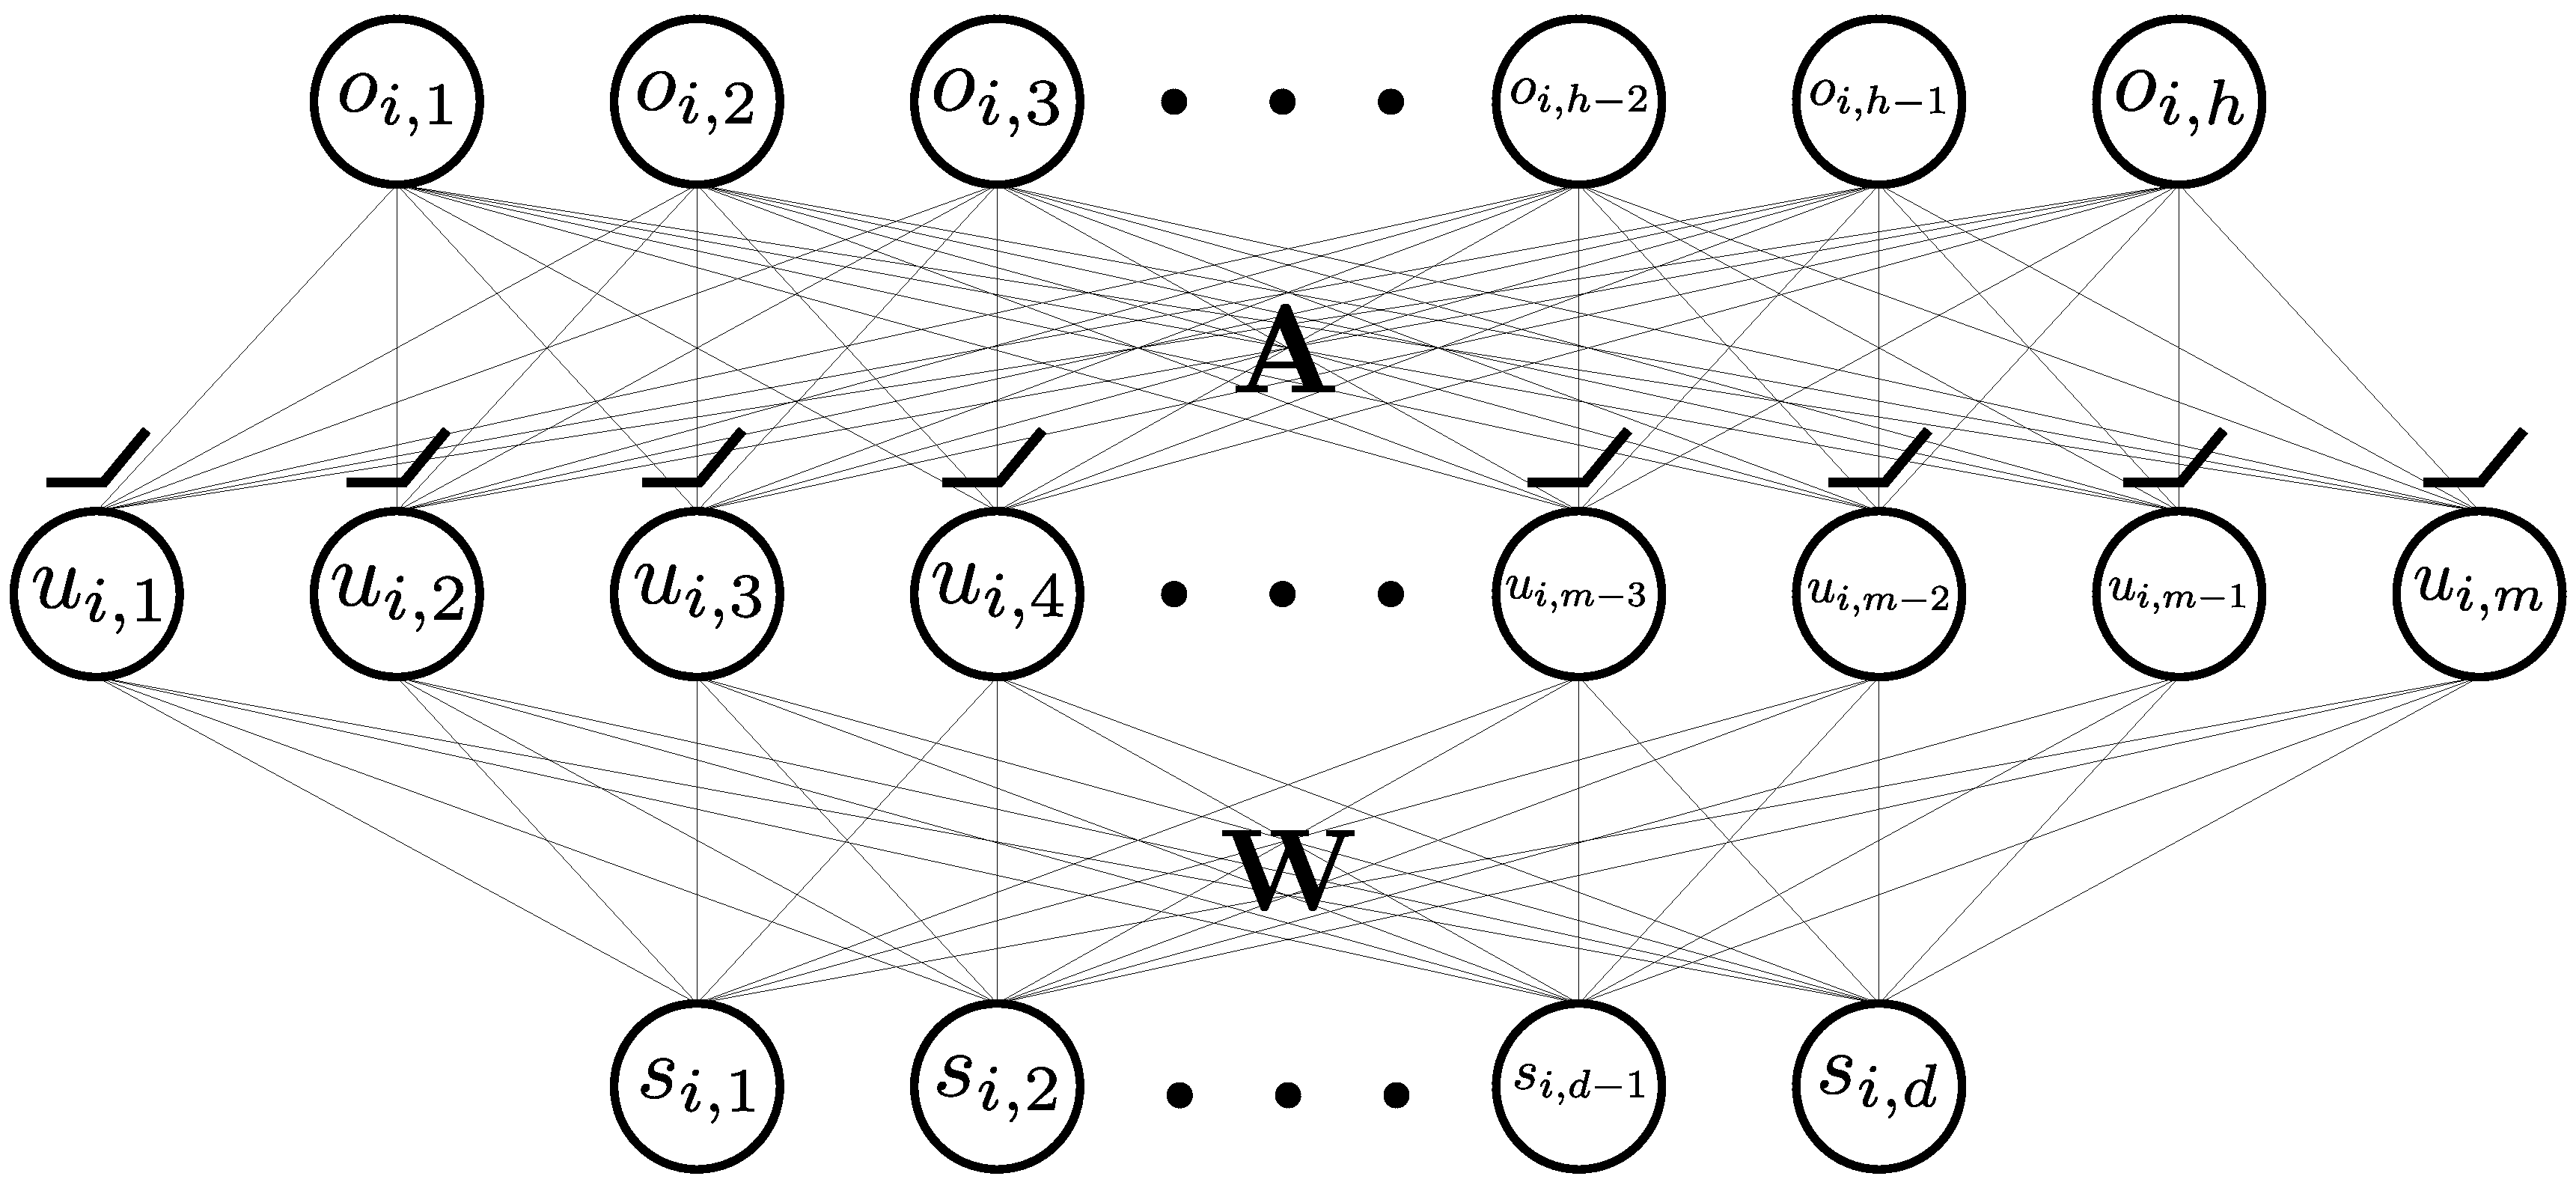
\includegraphics[width=\columnwidth]{nn_value.pdf}}
		\caption{Value neural network.}
		\label{fig:nn_value}
	\end{center}
	\vskip -0.2in
\end{figure}



%We mainly focus on the standard stochastic bandit setting with $n = 1$, i.e., there is only one state $\rvs_i$. At each time step $t$, the agent takes an action $A_t \in [h]$ according to its own strategies, and then it observes a random reward $R_{i, A_t} \in \sR$, where the mean value of $R_{i, A_t}$ is $r_{i, A_t}$. The agent then uses the reward to improve its action selection strategies. After such $T$ time steps, the performance of the agent's strategy is measured by the (expected) regret,
%\begin{equation}
%\label{eq:expected_regret}
%    \sum\limits_{t=0}^{T-1}{{\rvpi_i^*}^\top \rvr_i} - \sE \left[ \sum\limits_{t=0}^{T-1}{  r_{i, A_t}  } \right] = \sum\limits_{t=0}^{T-1}{{\rvpi_i^*}^\top \rvr_i} - \sum\limits_{t=0}^{T-1}{ \sE \left[ r_{i, A_t} \right] },
%\end{equation}
%where the expectation is over the randomness of action selection, if the agent is using some stochastic strategies.


\subsection{NEURAL NETWORK VALUE FUNCTION APPROXIMATION AND POLICY}
\label{subsec:nn_value_policy}
The structure of the value network and the policy network  is a 2-layers fully connected neural network with ReLU activation, as shown in \cref{fig:nn_value} and \cref{fig:nn_policy}, respectively. 
Each neural network takes the state $\rvs \in \sR^d$ as its input, where without loss of generality we assume that $\left\| \rvs \right\|_2 = 1$.
The hidden layer of both networks are denoted by $\rvu   \triangleq W\rvs\in\sR^m$, and the logit output $\rvo \triangleq A\sigma\left( \rvu\right) \in \sR^h$, where $\sigma$ is element-wise ReLU activation function. 
The policy network differs the value network with one additional softmax transform layer in order to output probability distributions, where $\rvpi \triangleq f\left( \rvo \right) = f\left( \rmA \sigma\left( \rmW \rvs \right) \right)$, and $f$ is the softmax function. In the rest of the paper we denote the policy $\rvpi$ by $\rvpi(\rmW)$ to emphasize its parametrization by $\rmW$. 

%Both the value and the policy neural networks take the state feature  $\rvs_i \in \sR^d$ as the input. Then the networks calculate the hidden node value vector by $u_{i,r} \triangleq \rvw_r^\top \rvs_i$, $\forall r \in [m]$. The logit vector is then calculated by $o_{i,k} \triangleq \rva_k^\top \sigma\left( \rvu_i \right)$, $\forall k \in [h]$, where $\sigma$ is element-wise ReLU activation function. The value neural network outputs the logit vector $\rvo_i$. While the policy neural network output probability is the softmax transform of the logit vector, i.e., $\rvpi_i \triangleq f\left( \rvo_i \right) = f\left( \rmA \sigma\left( \rmW \rvs_i \right) \right)$. 

\begin{figure}[t]
\vskip 0.2in
\begin{center}
\centerline{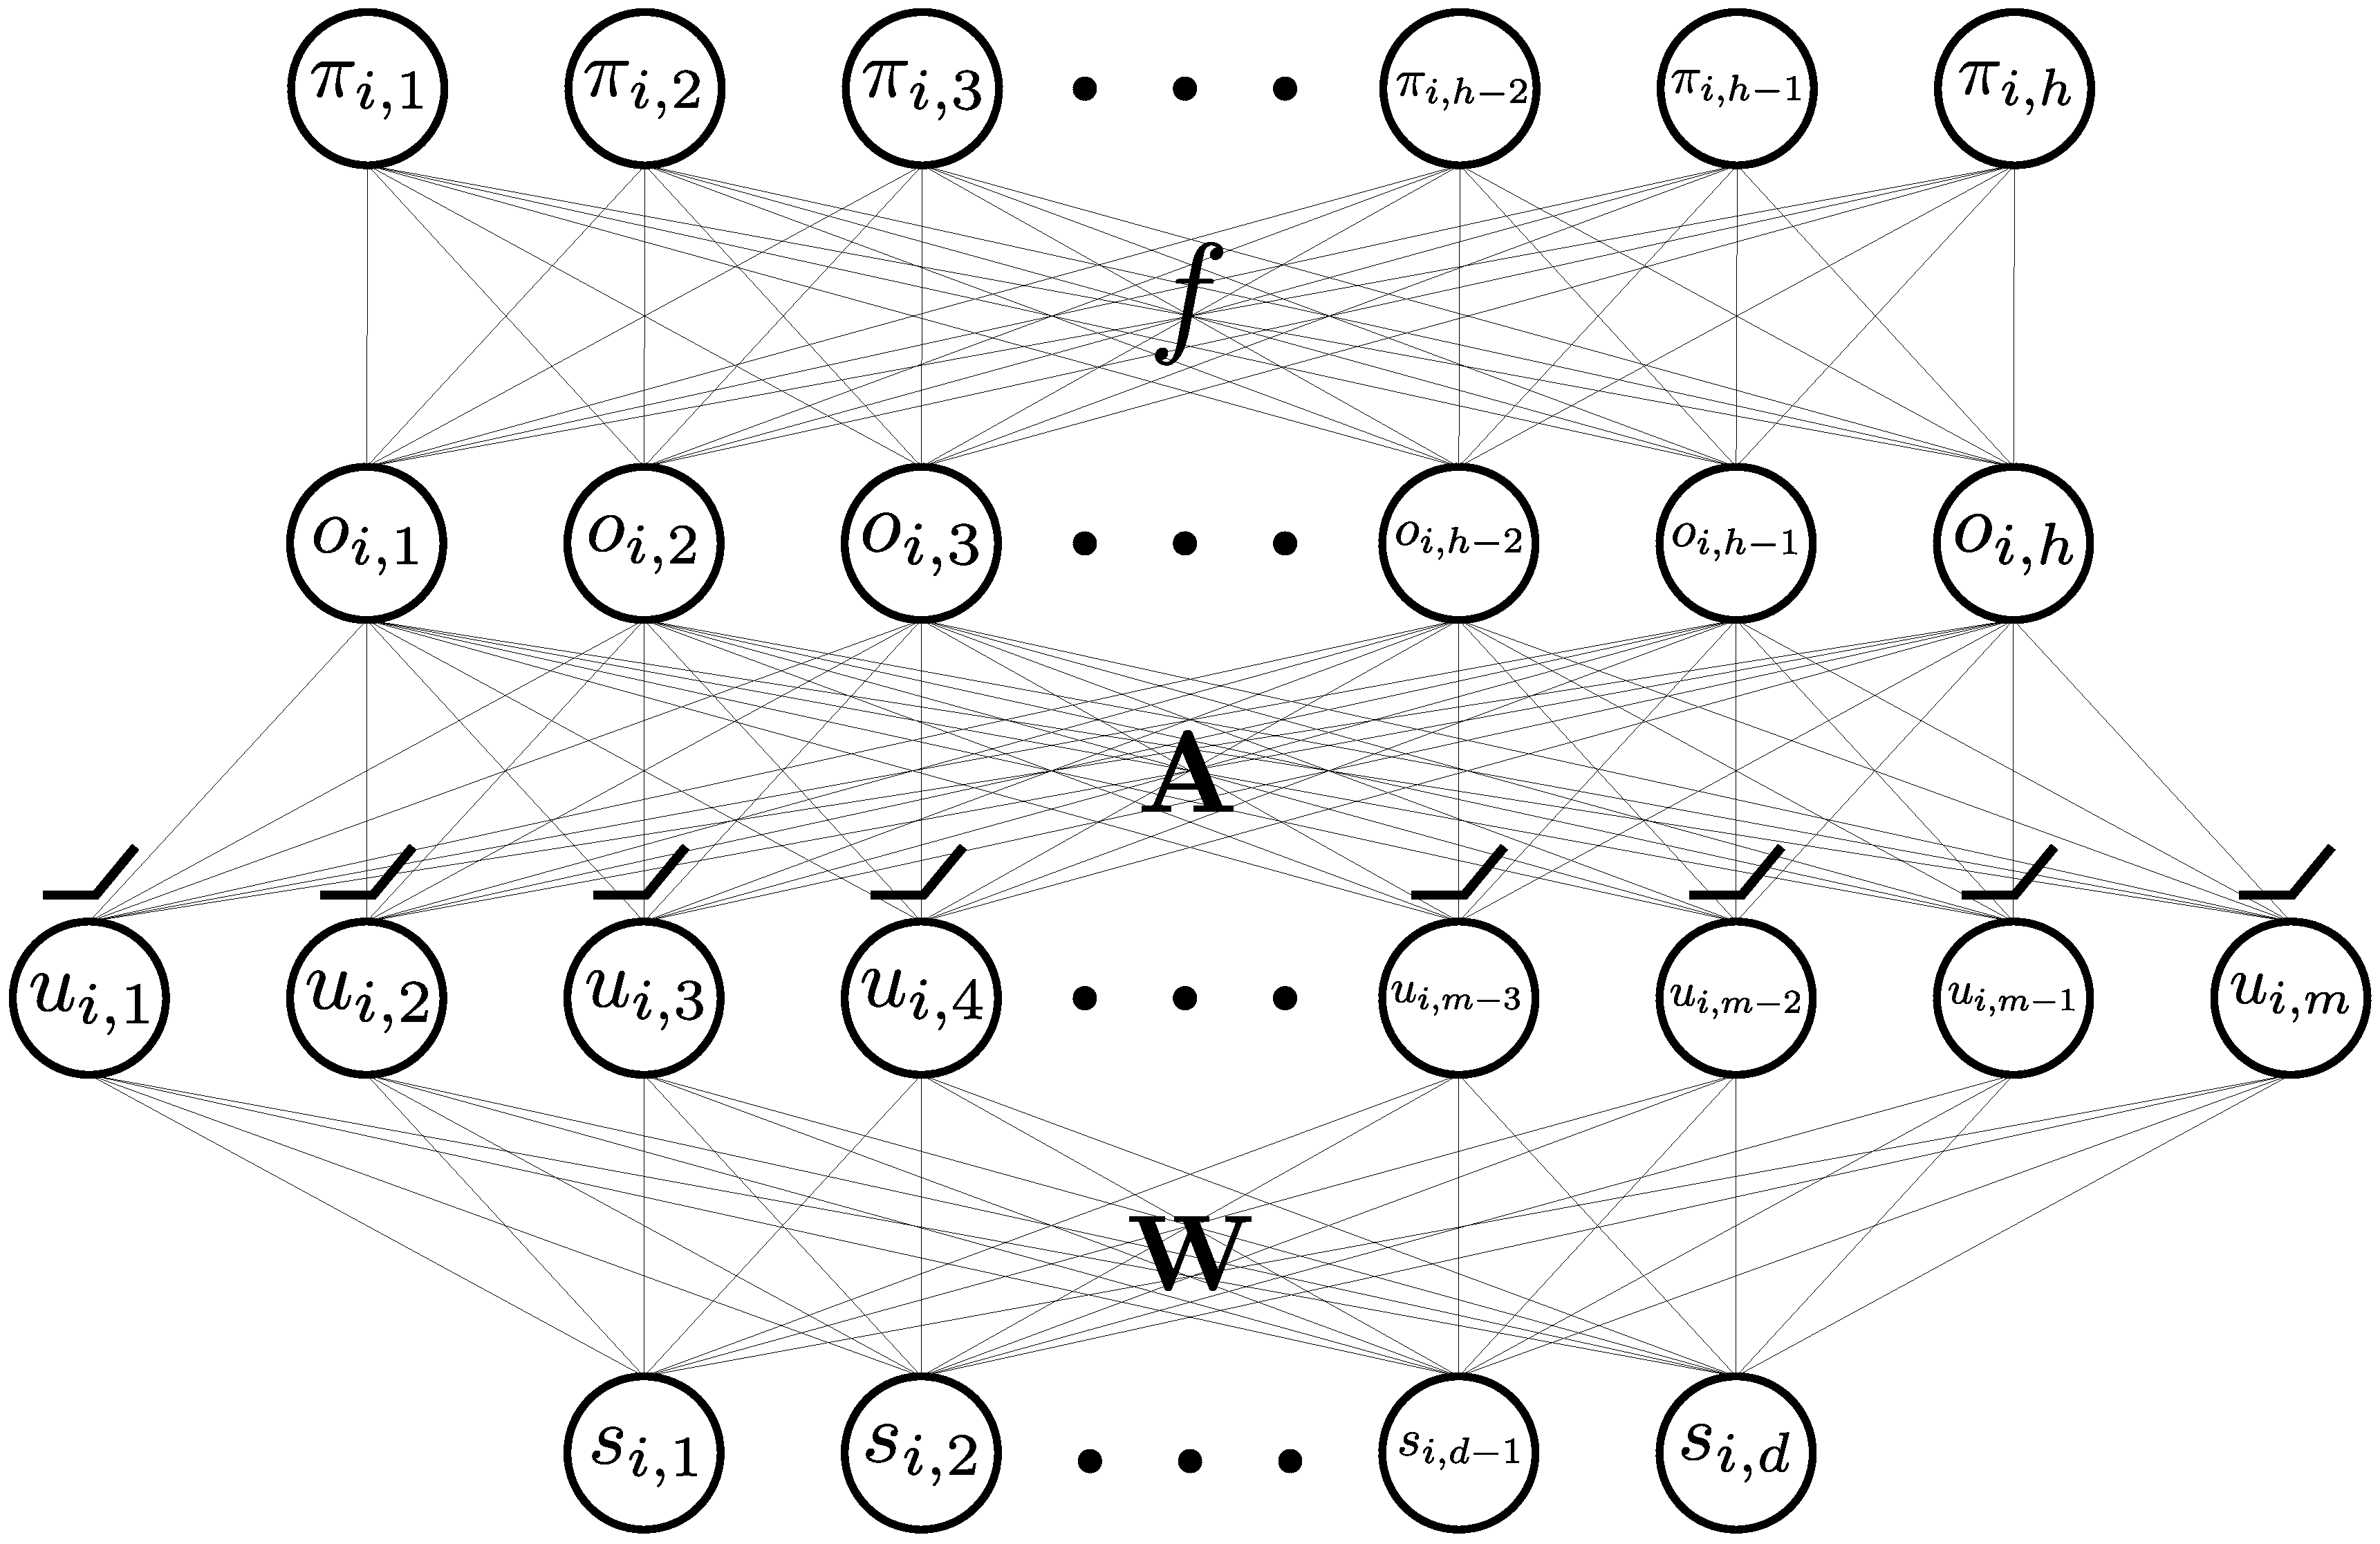
\includegraphics[width=\columnwidth]{nn_policy.pdf}}
\caption{Policy neural network.}
\label{fig:nn_policy}
\end{center}
\vskip -0.2in
\end{figure}

%The policy neural network defines a family of policies $\rvpi_i \left( \rmW \right)$ parameterized by $\rmW \in \sR^{m \times d}$ given any state $\rvs_i$. Let $\rvpi_i = \rvpi_i \left( \rmW \right)$, the expected loss of the policy neural network can be calculated according to \cref{eq:expected_loss}.

\paragraph{Multi-layered neural networks.} We would like to point that our algorithms and results can be easily extended to general value functions and policies parameterized by multi-layered neural networks \citep{allen2018convergenceA,allen2018convergenceB,du2018gradientA}. For the sake of simplicity and conciseness, we focus on two-layers neural networks in the paper.

%Although there is only one state, i.e., $n = 1$, and $i$ can be omitted without ambiguity, we choose to keep the subscript $i$ here to make the generalization from the standard bandit setting to the many state dependent setting smoother, and our algorithms work for general $n > 1$. For simplicity, we assume $\left\| \rvs_{i} \right\|_2 = 1$, $\forall i \in [n]$.

%In the case of $n > 1$, for each state $\rvs_i$, there is a state dependent policy $\rvpi_i$. And the agent's goal is to learn totally $n$ policies using only one neural network. We assume $\left\| \rvs_{i} -  \rvs_{j} \right\|_2 \ge \delta > 0 , \ \forall i \not= j$, i.e., no duplicated data, and $\left\| \rvs_{i} \right\|_2 = 1, \ \forall i \in [n]$.

\subsection{LOGIT LEARNING}
\label{subsec:logit_learning}

Our first proposed algorithm is Logit Learning with $\epsilon$-Greedy Exploration, as shown in \cref{alg:logit_learning_eps_greedy_exploration}. After the random initialization, at each time step $t$, the agent selects the action with the largest logit with probability $1 - \epsilon_t$, and it uniformly randomly select actions with the other probability $\epsilon_t$. After taking action and observing rewards, the agent improves its strategies by minimizing the value loss objective $\frac{1}{2} \left\| \rvo_i\left( \rmW\left(t\right)\right) - \hat{\rvr}_i\left(t\right) \right\|_2^2$, where $\hat{\rvr}_i\left(t\right)$ is the empirical mean reward estimated from sampled rewards up to step $t$. In each iteration, the agent only update its value neural network using one gradient descent, therefore the logit learning is in an online fashion.


\begin{algorithm}[t]
   \caption{Logit Learning with $\epsilon$-Greedy Exploration}
\label{alg:logit_learning_eps_greedy_exploration}
\begin{algorithmic}
   \STATE {\bfseries Input:} State feature $\rvs_i$, learning rate $\eta > 0$.
   \STATE $\rvw_r(0) \sim \gN\left( 0, \sigma^2 \cdot \rmI \right)$, $\forall r \in [m]$.
   \STATE $a_{k, r} \sim \gU\left\{-1, +1\right\}$, $\forall k \in [h]$, $\forall r \in [m]$.
   \STATE $\hat{r}_{i,k}\left(0\right) \gets 0$, $n_{i,k}\left(0\right) \gets 0$, $\forall k \in [h]$.
   \STATE $\hat{\Delta}_{i,k}\left(0\right) \gets \max\limits_{k^\prime}\left\{ \hat{r}_{i,k^\prime}\left(0\right) \right\} - \hat{r}_{i,k}\left(0\right)$, $\forall k \in [h]$.
   \STATE $\tilde{\Delta}_{i,k}\left(0\right) \gets \max\limits_{k^\prime}\left\{ o_{i,k^\prime}\left(0\right) \right\} - o_{i,k}\left(0\right)$, $\forall k \in [h]$.
   \FOR{$t=0$ {\bfseries to} $T-1$}
   \STATE $\xi_t \gets \frac{\log{t}}{t \hat{\Delta}_{i,k}^2\left(0\right)}$, $\epsilon_t \gets \min\left\{ \frac{1}{2 h}, \xi_t \right\}$.
   \STATE $\pi_{i, k}\left(t\right) \gets 1$, for $k = \argmax\limits_{k^\prime \in \left[h\right]}\left\{ o_{i, k^\prime}\left(t\right)\right\}$.
   \STATE $\pi_{i, k}\left(t\right) \gets 0$, $\forall k \not= \argmax\limits_{k^\prime \in \left[h\right]}\left\{ o_{i, k^\prime}\left(t\right)\right\}$.
   \STATE $\tilde{\rvpi}_i\left(t\right) \gets \left( 1 - \epsilon_t \right) \cdot  \rvpi_i\left(t\right) + \epsilon_t \cdot \gU{\left[ h \right]}$.
   \STATE Sample action $A_{t} \sim \tilde{\rvpi}_{i}\left(t\right)\left(\cdot \middle| \rvs_i \right)$.
   \STATE Take action $A_{t}$. Observe reward $R_{i, A_{t}}\left(n_{i, A_{t}}\left(t\right) \right)$.
   \STATE $n_{i, A_{t}}\left(t+1\right) \gets n_{i, A_{t}}\left(t\right) + 1$.
   \STATE $\hat{r}_{i,A_{t}}\left(t+1\right) \gets \frac{n_{i, A_{t}}\left(t\right) \cdot \hat{r}_{i,A_{t}}\left(t\right) + R_{i, A_{t}}\left(n_{i, A_{t}}\left(t\right)\right) }{n_{i, A_{t}}\left(t+1\right)}$.
   \STATE $n_{i, k}\left(t+1\right) \gets n_{i, k}\left(t\right)$, $\forall k \not= A_t$.
   \STATE $\hat{r}_{i,k}\left(t+1\right) \gets \hat{r}_{i,k}\left(t\right)$, $\forall k \not= A_t$.
   \STATE $\rmW(t+1) \leftarrow \rmW(t) - \eta \cdot \frac{d \left\{ \frac{1}{2} \left\| \rvo_i\left( \rmW\left(t\right)\right) - \hat{\rvr}_i\left(t\right) \right\|_2^2 \right\}}{d \rmW(t)}$.
   \ENDFOR
\end{algorithmic}
\end{algorithm}

\subsection{POLICY GRADIENT}
\label{subsec:policy_gradient}

Our second proposed algorithm is based on the widely used policy gradient method. Consider at each step $t$, the agent is using $\rvpi_i\left(\rmW(t)\right)$ as shown in \cref{fig:nn_policy} as its action selection strategy, then the (expected) regret is equivalent to the cumulative expected loss of $\rvpi_i\left(\rmW(t)\right)$, i.e., 
\begin{equation}
\label{eq:vanilla_policy_gradient_expected_regret}
\begin{split}
    &\sum\limits_{t=0}^{T-1}{{\rvpi_i^*}^\top \rvr_i} - \sum\limits_{t=0}^{T-1}{ \expectation\limits_{A_t \sim \rvpi_i\left(\rmW(t)\right)} \left[ r_{i, A_t} \right] } \\
    &= \sum\limits_{t=0}^{T-1}{{\rvpi_i^*}^\top \rvr_i} - \sum\limits_{t=0}^{T-1}{\rvpi_i\left(\rmW(t)\right)^\top \rvr_i},
\end{split}
\end{equation}
by \cref{eq:expected_loss} and \cref{eq:expected_regret}. Using \cref{eq:vanilla_policy_gradient_expected_regret}, at each time step $t$, the agent can use the current NN policy $\rvpi_i\left(\rmW(t)\right)$ to sample an action, and obtain an estimation of the expected loss $\rvpi_i\left(\rmW(t)\right)^\top \rvr_i$. Doing policy gradient updates with respect to the NN weights $\rmW(t)$ will arguably decrease the expected loss, thus reduce the expected regret. 

Unfortunately, the vanilla policy gradient often suffers the ``lack of exploration" problem in practice, i.e., some actions can never be explored thus cannot be learned. Therefore, we propose a two stage algorithm combining policy gradient with uniform exploration as shown in \cref{alg:policy_gradient_uniform_exploration}. After the random initialization, at each step $t$, one of the two cases happens. If $t < T^{\frac{2}{3} + \beta}$, then agent gets into a purely ``exploring phase", without learning the policy neural network, while just collecting empirically estimated rewards. If $t \ge T^{\frac{2}{3} + \beta}$, then the agent starts ``playing and learning". The agent samples and takes actions according to the current neural network policy $\rvpi_{i}\left(\rmW(t)\right)$. In the meanwhile, the agent learns the policy neural network by doing policy gradient updates, with the expected empirically estimated loss calculated from the exploring phase as its objective.

\begin{algorithm}[t]
   \caption{Policy Gradient with Uniform Exploration}
\label{alg:policy_gradient_uniform_exploration}
\begin{algorithmic}
   \STATE {\bfseries Input:} State feature $\rvs_i$, learning rate $\eta > 0$, $\beta > 0$.
   \STATE $\rvw_r(0) \sim \gN\left( 0, \sigma^2 \cdot \rmI \right)$, $\forall r \in [m]$.
   \STATE $a_{k, r} \sim \gU\left\{-1, +1\right\}$, $\forall k \in [h]$, $\forall r \in [m]$.
   \STATE $\hat{r}_{i,k}\left(0\right) \gets 0$, $n_{i,k}\left(0\right) \gets 0$, $\forall k \in [h]$.
   \FOR{$t=0$ {\bfseries to} $T-1$}
   \IF{$t < T^{\frac{2}{3} + \beta}$}
   \STATE (Exploring Phase)
   \STATE Uniformly randomly sample action $A_{t} \in [h]$.
   \STATE $\rmW(t+1) \leftarrow \rmW(t)$.
   \ELSE
   \STATE (Playing-Learning Phase)
   \STATE Sample action $A_{t} \sim \rvpi_{i}\left(\rmW(t)\right)\left(\cdot \middle| \rvs_i \right)$.
   \STATE $\rmW(t+1) \leftarrow \rmW(t) + \eta \cdot \frac{d \rvpi_{i}\left(\rmW(t)\right)^\top \hat{\rvr}_i \left(t\right)}{d \rmW(t)}$.
   \ENDIF
   \STATE Take action $A_{t}$. Observe reward $R_{i, A_{t}}\left(n_{i, A_{t}}\left(t\right) \right)$.
   \STATE $n_{i, A_{t}}\left(t+1\right) \gets n_{i, A_{t}}\left(t\right) + 1$.
   \STATE $\hat{r}_{i,A_{t}}\left(t+1\right) \gets \frac{n_{i, A_{t}}\left(t\right) \cdot \hat{r}_{i,A_{t}}\left(t\right) + R_{i, A_{t}}\left(n_{i, A_{t}}\left(t\right)\right) }{n_{i, A_{t}}\left(t+1\right)}$.
   \STATE $n_{i, k}\left(t+1\right) \gets n_{i, k}\left(t\right)$, $\forall k \not= A_t$.
   \STATE $\hat{r}_{i,k}\left(t+1\right) \gets \hat{r}_{i,k}\left(t\right)$, $\forall k \not= A_t$.
   \ENDFOR
\end{algorithmic}
\end{algorithm}

\paragraph{Initialization of the matrix $\mathbf{A}$.} Note that in \cref{alg:logit_learning_eps_greedy_exploration} and \cref{alg:policy_gradient_uniform_exploration}, after the random initialization $a_{k,r} \sim \gU\left\{-1, +1\right\}$, $a_{k,r}$ is fixed during learning, which is a common assumption in literature \citep{li2018learning,du2018gradientA,du2018gradientB,allen2018convergenceA,allen2018convergenceB}, and it has been empirically verified that there is no impact on the performance of trained neural networks \citep{hoffer2018fix}. Some other initializations like $\rva_k \sim \gN(0, \rmI)$ also work.


%\section{Theoretical Analysis}

\subsection{Main Results}
\label{subsec:main_results}

We first present the main results in the bandit setting, as shown in \cref{thm:main_result}, and defer the results of more general settings later.

\begin{thm}
\label{thm:main_result}
    Given a two layer NN policy $\rvpi_i$, with number of parameters $m \in \tilde{\Theta}\left( \frac{\log{T}}{c^4} \right)$, $\eta \in \Theta\left( \frac{c^2}{16 h m \left( \log{\left(4m\right)} \right)^2} \right)$, the expected regret of \cref{alg:policy_gradient_uniform_exploration} satisfies $\sum\limits_{t=0}^{T-1}{ \sE \left[ \tilde{r}_{i, A_t} \right] } \le  \frac{8\sqrt{h}}{c^2} \cdot \tilde{O}\left( \sqrt{T} \right)$.
\end{thm}
\begin{proof}
According to \cref{alg:policy_gradient_uniform_exploration}, the agent uniformly samples and takes actions in the exploring phase, which leads to at most $\sqrt{T}$ regret. At the end of the exploring phase, each action is taken $\frac{\sqrt{T}}{h}$ times in expectation, by \cref{thm:regret_convergence}, 
\begin{equation*}
\begin{split}
    \rvpi_i\left( \rmW(t) \right)^\top \rvtilder_i \le O\left( \frac{n^4}{\eta m c^2 \delta^2 \sqrt{T}} \right),
\end{split}
\end{equation*}
for $t = \sqrt{T}$. Denote $\varepsilon \triangleq \frac{n^4}{\eta m c^2 \delta^2 \sqrt{T}}$. By \cref{subsec:playing_phase}, $\rvpi_i\left( \rmW(t) \right)^\top \rvtilder_i \le \varepsilon$, $\forall t \ge \sqrt{T}$. Therefore the regret can be upper bounded by the sum of two parts,
\begin{equation*}
\begin{split}
    \sum\limits_{t=0}^{T-1}{ \sE \left[ \tilde{r}_{i, A_t} \right] } &\le \sum\limits_{t=0}^{\sqrt{T}-1}{ 1 } + \sum\limits_{t=\sqrt{T}}^{T-1}{ \rvpi_i\left( \rmW(t) \right)^\top \rvtilder_i } \\
    &\le \sqrt{T} + \left( T - \sqrt{T} \right) \varepsilon \\
    &\le \frac{8 n^4 \sqrt{h}}{c^2 \delta^2} \cdot \log{\left(4m\right)} \cdot \sqrt{T} \\
    &\le \frac{8 n^4 \sqrt{h}}{c^2 \delta^2} \cdot \tilde{O}\left(\sqrt{T}\right). \qedhere
\end{split}
\end{equation*}
\end{proof}

\cref{alg:policy_gradient_uniform_exploration} divides $T$ steps into two parts. In the first $\sqrt{T}$ exploring phase steps, the agent uniformly samples actions, and learnd the NN policy with expected loss convergent to smaller than $\varepsilon$. Intuitively, this phase is necessary because of: (a) unlike tabular algorithms, i.e., maintaining a scalar value for each arm, the NN policy evolves in a much slower way, due to the usually very small learning rate $\eta$; (b) it is sufficient that the expected loss of the the NN policy is small enough, to make the NN policy have large enough probability for the optimal arm. While in the second playing phase, because of the expected loss of the NN policy is small enough, the gradient norm will be lower bounded by positive constant times expected loss. Therefore the NN policy will keep reducing its expected loss, which means the expected regret will also be reduced. Our detailed analysis also consists of corresponding two parts.

\subsection{Exploring Phase}
\label{subsec:exploring_phase}

As aforementioned, the agent need to learn a good enough NN policy at the end of the exploring phase. The performance of the NN policy can be measured by its expected loss \cref{eq:expected_loss}. And the convergence of the expected loss relies on the following ``smoothness" like property over local change of the NN weights.

\begin{lem}
\label{lem:smoothness}
    Given weights $\rmW \triangleq \left[ \rvw_1, \rvw_2, \dots, \rvw_m \right]$, and $\rmW^\prime \triangleq \left[ \rvw_1^\prime, \rvw_2^\prime, \dots, \rvw_m^\prime \right]$. Denote $\rvpi_i\left( \rmW \right)$ and $\rvpi_i\left( \rmW^\prime \right)$ as the neural network policies parameterized by $\rmW$ and $\rmW^\prime$, respectively. $\forall i \in [n]$,
\begin{equation*}
\begin{split}
    &\rvpi_i\left( \rmW^\prime \right)^\top \rvtilder_i \le \rvpi_i\left( \rmW \right)^\top \rvtilder_i + \left\langle \frac{d \rvpi_i\left( \rmW \right)^\top \rvtilder_i }{d\left( \rmW \right)}, \rmW^\prime - \rmW \right\rangle \\
    &\qquad + 4 \sqrt{m \log{\left(4m\right)}} \cdot \rvpi_i\left( \rmW \right)^\top \rvtilder_i \cdot \left\| \rmW^\prime - \rmW \right\|_F \\
    &\qquad + 4 h m \log{\left(4m\right)} \cdot \left\| \rmW^\prime - \rmW \right\|_F^2.
\end{split}
\end{equation*}
\end{lem}

Usually, combining this smoothness condition with other objective properties like convexity, one can prove convergence results. However, the policy expected loss is non-convex over NN weights. We resort to the recent progresses in the overparameterized NN optimization theory, i.e., the gradient coupling and gradient lower bounds \citep{li2018learning}.

\begin{lem}
\label{lem:gradient_coupling}
	Define the pseudo policy gradient as,
\begin{equation*}
\begin{split}
	\frac{d \tilde{\ell}}{d \rvw_r(t)} &\triangleq \frac{1}{n} \cdot \sum\limits_{i=1}^{n}{ \sum\limits_{k=1}^{h}{ \tilde{r}_{i,k} \cdot \pi_{i,k}(t) \cdot \left( \sum\limits_{k^\prime = 1}^{h}{ a_{k^\prime,r}  \cdot v_{k^\prime,k,i}(t) } \right) } } \\
	&\qquad { { \cdot \sI\left\{ \rvw_r(0)^\top \rvs_i > 0 \right\} \cdot \rvs_i } },
\end{split}
\end{equation*}
where $v_{k^\prime,k,i}(t)$ is defined as,
\begin{equation*}
	v_{k^\prime,k,i}(t) = \begin{cases}
    1 - \pi_{i,k^\prime}(t), & \text{if $k^\prime = k$}, \\
    - \pi_{i,k^\prime}(t), & \text{otherwise}.
  \end{cases}
\end{equation*}
	For any $\tau > 0$, with probability at least $\frac{1}{2} \cdot \left( 1 - \frac{\sqrt{2}n\tau}{\sqrt{\pi}\sigma} \right)$, $\forall t \in O\left(\frac{\tau}{\eta  \sqrt{\log{m}}}\right)$, $\forall r \in [m]$,
\begin{equation}
	\frac{d\ell}{d \rvw_r(t)} = \frac{d \tilde{\ell}}{d \rvw_r(t)},
\end{equation}
where $\frac{d\ell}{d \rvw_r(t)}$ is the true policy gradient,
\begin{equation*}
\begin{split}
    \frac{d\ell}{d \rvw_r(t)} &= \frac{1}{n} \cdot \sum\limits_{i=1}^{n}{ \sum\limits_{k=1}^{h}{  \tilde{r}_{i,k} \cdot \pi_{i,k}(t) \cdot \left( \sum\limits_{k^\prime = 1}^{h}{ a_{k^\prime,r}  \cdot v_{k^\prime,k,i}(t) } \right) }} \\
    &\qquad  {{ \cdot \sI\left\{ \rvw_r(t)^\top \rvs_i > 0 \right\} \cdot \rvs_i } }.
\end{split}
\end{equation*}
\end{lem}

\cref{lem:gradient_coupling} implies that with constant probability, for bounded numbers of policy gradient updates, the signs of the true policy gradient will not change, i.e., $\sI\left\{ \rvw_r(t)^\top \rvs_i > 0 \right\} = \sI\left\{ \rvw_r(0)^\top \rvs_i > 0 \right\}$, thus the true gradient is equal to the pseudo gradient, which is easy to be analyzed and it has nice relationship with the expected loss \cref{lem:gradient_lower_bound}.

The next lemma shows that the true policy gradient norm is upper bounded by the expected loss.

\begin{lem}
\label{lem:gradient_upper_bound}
With probability at least $\frac{1}{2}$,
\begin{equation*}
\begin{split}
	\left\| \frac{d\ell}{d \rvw_r(t)} \right\|_2 \le 2 \sqrt{\log{\left(4m\right)}} \cdot \rvpi_{i}(t)^\top \rvtilder_i.
\end{split}
\end{equation*}
\end{lem}

Now comes the key insight of the recent progresses of the overparameterized NN optimization theory. With constants probability, the pseudo policy gradient norm is lower bounded by the expected loss. However, due to the inherent difference between RL and supervised learning, our result contains an exploration related term, which directly leads to the necessity of the exploring phase in \cref{alg:policy_gradient_uniform_exploration}. 

\begin{lem}
\label{lem:gradient_lower_bound}
	Denote $i^*(t) \triangleq \argmax\limits_{i \in [n]}\left\{\rvpi_i(t)^\top \rvtilder_i \right\}$, $k^*(t) \triangleq \argmax\limits_{k \in [h]}\left\{ r_{i^*(t),k} \right\} = \r_{i^*(t)}^{\max}$, i.e., the optimal arm of state $\rvs_{i^*(t)}$. If $\pi_{i^*(t), k^*(t)}(t) > c_t > 0$, then with probability at least $\Omega\left( \frac{\delta}{n} \right)$,
\begin{equation*}
\begin{split}
	\left\| \frac{d\tilde{\ell}}{d \rvw_r(t)} \right\|_2 \ge \Omega\left( \frac{\delta}{n^2} \right) \cdot c_t \cdot  \rvpi_{i^*(t)}(t)^\top \rvtilder_{i^*(t)}.
\end{split}
\end{equation*}
\end{lem}

\cref{lem:gradient_lower_bound} is a generalization of recent overparameterized NN optimization results into the RL field. By \cref{lem:gradient_lower_bound}, whenever the policy expected loss $\rvpi_{i^*(t)}(t)^\top \rvtilder_{i^*(t)}$ is large, with enough exploration of the optimal action (the term $c_t > 0$ here), with constant probability, the pseudo policy gradient norm will also be large. Therefore, combining \cref{lem:gradient_lower_bound} with \cref{lem:gradient_coupling}, we can get the true policy gradient norm is also large, which is necessary for making progresses to reduce the policy expected loss. Carefully applying all the stated results, we get the policy expected loss convergence result for the exploring phase.

\begin{thm}
\label{thm:regret_convergence}
    Let $\rvpi_i\left( \rmW(t) \right)$ be the NN policy parameterized by the weights $\rmW$. Assume $m \in \tilde{\Theta}\left( \frac{n^{10}}{c^4 \delta^4 \varepsilon^2} \right)$, $\eta \in \Theta\left( \frac{c^2 \delta^2}{16 n^4 h m \left( \log{\left(4m\right)} \right)^2} \right)$, after $t \in O\left( \frac{n^4}{\eta m c^2 \delta^2 \varepsilon} \right)$ policy gradient descent iterations, $\rvpi_i\left( \rmW(t) \right)^\top \rvtilder_i \le \varepsilon$.
\end{thm}
\begin{proof}
    By \cref{lem:gradient_coupling}, let $\tau = \frac{\sigma}{n}$, there are $\Omega\left( m \right)$ of $\rvw_r(t)$ such that $\left\| \frac{d\ell}{d \rvw_r(t)} \right\|_2 = \left\| \frac{d\tilde{\ell}}{d \rvw_r(t)} \right\|_2$, $\forall t \in O\left( \frac{\sigma}{\eta n \sqrt{\log{m}}} \right)$. Let $\rmW(t+1) = \rmW(t) - \eta \cdot \frac{d \ell}{d \rmW(t)}$, by \cref{lem:smoothness},
\begin{equation*}
\begin{split}
    &\rvpi_i\left( \rmW(t+1) \right)^\top \rvtilder_i \le \rvpi_i\left( \rmW(t) \right)^\top \rvtilder_i - \eta \cdot \left\| \frac{d \ell}{d \rmW(t)} \right\|_F^2 \\
    &\qquad + 4 \sqrt{m \log{\left(4m\right)}} \cdot \rvpi_i\left( \rmW \right)^\top \rvtilder_i \cdot \eta \cdot \left\| \frac{d \ell}{d \rmW(t)} \right\|_F \\
    &\qquad + 4 h m \log{\left(4m\right)} \cdot \eta^2 \left\| \frac{d \ell}{d \rmW(t)} \right\|_F^2 \\
    &\le \rvpi_i\left( \rmW(t) \right)^\top \rvtilder_i - \eta \cdot \sum\limits_{r=1}^{m}{ \left\| \frac{d\ell}{d \rvw_r(t)} \right\|_2^2 } \\
    &\qquad + 4 \sqrt{m \log{\left(4m\right)}} \cdot \rvpi_i\left( \rmW \right)^\top \rvtilder_i \cdot \eta \cdot \sum\limits_{r=1}^{m}{ \left\| \frac{d\ell}{d \rvw_r(t)} \right\|_2 } \\
    &\qquad + 4 h m \log{\left(4m\right)} \cdot \eta^2 \cdot \sum\limits_{r=1}^{m}{ \left\| \frac{d\ell}{d \rvw_r(t)} \right\|_2^2 } \\
    &\le \rvpi_i\left( \rmW(t) \right)^\top \rvtilder_i - \left( \rvpi_i\left( \rmW(t) \right)^\top \rvtilder_i \right)^2 \\
    &\cdot \left[ \frac{\eta m c^2 \delta^2}{n^4} - 8 \eta m \sqrt{m} \log{\left(4m\right)} - 16 \eta^2 h m^2 \left( \log{\left(4m\right)} \right)^2 \right] \\
    &= \rvpi_i\left( \rmW(t) \right)^\top \rvtilder_i - \left( \rvpi_i\left( \rmW(t) \right)^\top \rvtilder_i \right)^2 \cdot \Omega\left( \frac{\eta m c^2 \delta^2}{n^4} \right).
\end{split}
\end{equation*}
Divide $\left( \rvpi_i\left( \rmW(t+1) \right)^\top \rvtilder_i\right) \cdot \left( \rvpi_i\left( \rmW(t) \right)^\top \rvtilder_i \right)$,
\begin{equation*}
\begin{split}
    &\frac{1}{\rvpi_i\left( \rmW(t+1) \right)^\top \rvtilder_i} - \frac{1}{\rvpi_i\left( \rmW(t) \right)^\top \rvtilder_i} \ge \\
    &\frac{\rvpi_i\left( \rmW(t) \right)^\top \rvtilder_i}{\rvpi_i\left( \rmW(t+1) \right)^\top \rvtilder_i} \cdot \Omega\left( \frac{\eta m c^2 \delta^2}{n^4} \right) \ge \Omega\left( \frac{\eta m c^2 \delta^2}{n^4} \right).
\end{split}
\end{equation*}
Sum up the inequality from $0$ to $t$,
\begin{equation*}
\begin{split}
    \frac{1}{\rvpi_i\left( \rmW(t) \right)^\top \rvtilder_i} \ge \Omega\left( \frac{\eta m c^2 \delta^2}{n^4} \right) \cdot t.
\end{split}
\end{equation*}
After $t \in O\left( \frac{n^4}{\eta m c^2 \delta^2 \varepsilon} \right)$ iterations, $\rvpi_i\left( \rmW(t) \right)^\top \rvtilder_i \le \varepsilon$. Let $\frac{n^4}{\eta m c^2 \delta^2 \varepsilon} \le \frac{\sigma}{n \eta \sqrt{\log{m}}} = \frac{1}{n \eta \sqrt{m \log{m}}}$, we have $m \ge \frac{n^{10}}{c^4 \delta^4 \varepsilon^2}\log{\left( \frac{n^{10}}{c^4 \delta^4 \varepsilon^2} \right)}$.
\end{proof}

\subsection{Playing Phase}
\label{subsec:playing_phase}

In this phase, we use the NN policy net to select actions and collect rewards. We still need to use the  results in \cref{subsec:exploring_phase} to make sure that the expected regret of running policies will not deteriorate. Fortunately, because of the enough exploration phase, we have the exploration item $c$ large enough.

\begin{lem}
    $c > 1 - \frac{1}{\Delta \sqrt{T}}$.
\end{lem}

With this result and \cref{subsec:exploring_phase}, we can prove that the objective progress is always positive and therefore the policy regret will be always less than $\varepsilon$ in the last $T - \sqrt{T}$ time steps. That is why we can safely use the NN policy to play without worrying lack of exploration issue.

\section{Generalizations}

\subsection{State Dependent Bandits}

\subsection{MDPs}

\subsection{Multi-Layered NN Policies}

\section{Related Work}




\if0
% In the unusual situation where you want a paper to appear in the
% references without citing it in the main text, use \nocite
\nocite{langley00}
\fi

\if0
\begin{table}[t]
\caption{Classification accuracies for naive Bayes and flexible
Bayes on various data sets.}
\label{sample-table}
\vskip 0.15in
\begin{center}
\begin{small}
\begin{sc}
\begin{tabular}{lcccr}
\toprule
Data set & Naive & Flexible & Better? \\
\midrule
Breast    & 95.9$\pm$ 0.2& 96.7$\pm$ 0.2& $\surd$ \\
Cleveland & 83.3$\pm$ 0.6& 80.0$\pm$ 0.6& $\times$\\
Glass2    & 61.9$\pm$ 1.4& 83.8$\pm$ 0.7& $\surd$ \\
Credit    & 74.8$\pm$ 0.5& 78.3$\pm$ 0.6&         \\
Horse     & 73.3$\pm$ 0.9& 69.7$\pm$ 1.0& $\times$\\
Meta      & 67.1$\pm$ 0.6& 76.5$\pm$ 0.5& $\surd$ \\
Pima      & 75.1$\pm$ 0.6& 73.9$\pm$ 0.5&         \\
Vehicle   & 44.9$\pm$ 0.6& 61.5$\pm$ 0.4& $\surd$ \\
\bottomrule
\end{tabular}
\end{sc}
\end{small}
\end{center}
\vskip -0.1in
\end{table}
\fi

%\section{General Settings}
\label{sec:general_settings}

Although the stochastic bandit setting is an oversimplified RL environment, it captures the trade off between exploration and exploitation, which is the intrinsic nature of many more complicated RL tasks. Beyond the stochastic bandit setting, our results can be easily generalized to the following more general settings with minimal efforts.

\subsection{Episodic Markov Decision Processes (MDPs)}

Each action in the standard bandit setting can be viewed as a special trajectory with length $H = 1$ in the episodic MDPs. In general with $H > 1$, \cref{alg:logit_learning_eps_greedy_exploration} can achieve similar result, with the total trajectory number changing from $h$ to $h^H$.
\begin{thm}
\label{thm:episodic_mdp_setting}
     Suppose $m \in \Theta\left( \frac{T^2}{c^4 h^{2H}} \right)$, $\eta = \frac{ 1 }{16 h m}$, the expected regret of \cref{alg:logit_learning_eps_greedy_exploration} satisfies $\sum\limits_{t=0}^{T-1}{ \sE \left[ r\left(A_t\right) \right] } \le C + \sum\limits_{k \in [h^H] : \Delta(k) > 0}{ \frac{ 3 \beta \left( \ln{T} \right)^2}{\Delta^2(k)} }  + \frac{ 3 \ln{T}}{h^H}$.
\end{thm}

The number of terms in the summation has an undesirable exponential dependence of trajectory length $H$. This seems cannot be eliminated by policy based RL methods, without taking advantage of the intermediate rewards in value based RL methods, such as Q-Learning \citep{jin2018q}. It is open whether value based RL methods enjoy nice theoretical guarantees with neural network function approximations.

\subsection{State Dependent Bandit Setting}

The standard stochastic bandit setting is a special case of the many state dependent bandit setting, with $n = 1$ and $\delta = 1$. Firstly, all the intermediate results work for general $n > 0$, including the $n > 1$ case.
For $n > 1$ and $\delta > 0$, we slightly modify \cref{alg:logit_learning_eps_greedy_exploration}, by setting the objective as the sum of all the $n$ terms. Consider the average expected loss over all the states, the regret results are similar with \cref{thm:logit_learning_main_result}, up to an additional factor $n$, can be easily reproduced.
\begin{thm}
\label{thm:many_state_dependent_bandit_setting}
     Supose $m \in \Theta\left( \frac{n^{10} T^2}{c^4 \delta^4 h^2} \right)$, $\eta = \frac{c^2 \delta^2}{16 n^4 h m}$, the expected regret of \cref{alg:logit_learning_eps_greedy_exploration} satisfies $\sum\limits_{t=0}^{T-1}{ \sE \left[ r_i\left(A_t\right) \right] } \le C + \sum\limits_{k \in [h^H] : \Delta(k) > 0}{ \frac{ 3 \beta n^8 \left( \ln{T} \right)^2}{c^4 \delta^4 \Delta^2(k)} }  + \frac{ 3 n \ln{T}}{h}$.
\end{thm}




%\section{Future Work}
\label{sec:future_work}

Our results are just at the beginning of theoretically understanding DRL. There are many problems remain open along this line.
\begin{itemize}
    \item The first open problem would be a policy based algorithm that can achieve $O(\ln T)$ regret. \cref{alg:policy_gradient_uniform_exploration} only achieves a $\tilde{O}(T^{2/3})$ regret. We hypothesize that a better rate should be achievable with a better analysis and less exploration in \cref{alg:policy_gradient_uniform_exploration}. 
    Especially such better analysis should be able to leverage the property that the algorithm needs not to have an small estimation error $\|\hat{\rvr} - \rvr\|_\infty$ to pick the optimal action.
    \item In this paper we only consider the $\epsilon$-greedy for exploration, which may not be optimal. Other exploration strategies, like count based exploration \cite{auer2002finite}, EXP3 \citep{seldin2014one}, posterior sampling \citep{agrawal2012analysis} 
    may be able to improve the current regret rates. Especially, with other type of exploration, can \cref{alg:logit_learning_eps_greedy_exploration} be improved to achieve an $O(\ln T)$ regret.
    \item Our current algorithms need to memorize the empirical mean reward for each pair of state and action, which is not viable for large scale problems in practice. Instead, most of the practical RL algorithms use the sampled reward at the current step, instead of the empirical mean, as an approximation of the true reward. Can we still prove similar regrets for the current reward.
    \item In practice, it can always be found that gradient updates travel a long distance rather than around initialization \citep{liu2018deeptracker}. And usually, practical NNs do not have that much overparamerized scales. Further progresses in the DL theory would be helpful for improving our current analyses of DRL.
    \item One interpretation of the last softmax layer could be from the maximum entropy policy optimization, where the softmax function is the optimizer of the expected reward with an entropy regularizer\cite{nachum2017bridging}. In this perspective, mirror descent seems to be a more natural optimizer compared to gradient descent. Could a mirror descent optimizer leads to a better regret rate in our current setting?
    \item We have just investigated the vanilla policy based and value based algorithms. Can our results be extended to other successful RL algorithms including value based and actor critic methods, e.g, DQN \cite{mnih2015human}, A3C \citep{mnih2016asynchronous}, and PCL \citep{nachum2017bridging}, etc.
    %\item For policy leaning with NN function approximations, there is no known lower bound, although at least the general $\Omega\left(\sqrt{T}\right)$ lower bound holds. We can get some sense from the two parts of the regret in \cref{thm:policy_gradient_main_result}. The NN learning part seems cannot be improved, since this is the best one can obtain under smoothness like properties and gradient upper $\&$ lower bounds. While the other exploration and estimation error part seems still have space to be improved. But whether $\Omega\left(\sqrt{T}\right)$ is achievable is still unknown.
\end{itemize}

\if0
% In the unusual situation where you want a paper to appear in the
% references without citing it in the main text, use \nocite
\nocite{langley00}
\fi

%\section{Conclusions}
\label{sec:conclusions}

In this paper, we provide finite time regret analysis of basic policy gradient method under the stochastic bandit setting, where the policy is represented by neural network function approximations. The main result is $O\left( T^{\frac{2}{3} + \beta} \right)$, $\forall \beta > 0$. The results can be generalized to many state dependent bandit settings, episodic MDPs, and can be combined with multi-layered neural network function approximations. Our findings are at the starting point of understanding more perspectives and providing theoretical supports for deep reinforcement learning.

\if0
\begin{table}[t]
\caption{Classification accuracies for naive Bayes and flexible
Bayes on various data sets.}
\label{sample-table}
\vskip 0.15in
\begin{center}
\begin{small}
\begin{sc}
\begin{tabular}{lcccr}
\toprule
Data set & Naive & Flexible & Better? \\
\midrule
Breast    & 95.9$\pm$ 0.2& 96.7$\pm$ 0.2& $\surd$ \\
Cleveland & 83.3$\pm$ 0.6& 80.0$\pm$ 0.6& $\times$\\
Glass2    & 61.9$\pm$ 1.4& 83.8$\pm$ 0.7& $\surd$ \\
Credit    & 74.8$\pm$ 0.5& 78.3$\pm$ 0.6&         \\
Horse     & 73.3$\pm$ 0.9& 69.7$\pm$ 1.0& $\times$\\
Meta      & 67.1$\pm$ 0.6& 76.5$\pm$ 0.5& $\surd$ \\
Pima      & 75.1$\pm$ 0.6& 73.9$\pm$ 0.5&         \\
Vehicle   & 44.9$\pm$ 0.6& 61.5$\pm$ 0.4& $\surd$ \\
\bottomrule
\end{tabular}
\end{sc}
\end{small}
\end{center}
\vskip -0.1in
\end{table}
\fi

\subsection{Policy Mirror Descent}
\label{sec:pmd}
We first present a basic policy optimization algorithm based on the idea of Mirror Descent (MD). MD has been widely used in the literature of online learning and constrained optimization problems \cite{nemirovskii1983problem,beck2003mirror}. In particular, given a \emph{reference policy} $\refPi$, let 
\[
\ENT(\pi_\theta; \tau, \refPi) = { \ep\limits_{\rho \sim \pi_\theta}{  r(\rho)  - \tau \KL(\pi_\theta \| \refPi) } }.
\]
The MD update for policy optimization problem is 
\begin{equation}
\label{eq:max_expected_reward_plus_relative_entropy}
\pi_{\theta_{t+1}} = \argmax\limits_{\pi_\theta \in \Pi}  \ENT(\pi_\theta; \tau, \pithetat), 
\end{equation}
which combines the expected reward \cref{max_expected_reward} with a relative entropy regularizer.
Similar ideas have also been explored in \cite{peters2007reinforcement,wierstra2008episodic,peters2010relative,schulman2015trust,montgomery2016guided,nachum2017trust,haarnoja2018soft,abdolmaleki2018maximum}. The following \cref{prop:mirrordescent_projection} suggests an efficient implementation of the mirror descent algorithm.

\begin{prop}
	\label{prop:mirrordescent_projection}
	Given a \emph{reference policy} $\refPi$, define $\bar{\pi}_\tau^*(\rho) =  \frac{\refPi(\rho) \exp\left\{ r(\rho) / \tau \right\}}{ \sum_{\rho^{\prime}}{\refPi(\rho^{\prime}) \exp\left\{ r(\rho^{\prime}) / \tau \right\} } }$, then
	\[
	\argmax\limits_{\pi_\theta \in \Pi}{\ENT(\pi_\theta; \tau, \refPi)}= \argmin\limits_{\pi_\theta \in \Pi}{ \KL(\pi_\theta \| \bar{\pi}_\tau^*) } ,
	\]
\end{prop}
%\vspace{-0.2in}
\begin{proof}
	$-\tau \KL(\pi_\theta \| \bar{\pi}_\tau^*) = - \tau \sum_{\rho}{ \pi_\theta(\rho) \log \pi_\theta(\rho) } + \tau \sum_{\rho}{ \pi_\theta(\rho) (\log \refPi(\rho) + r(\rho) / \tau ) }  - Z_{\refPi} = \ep_{\rho \sim \pi_\theta}{  r(\rho)  - \tau \KL(\pi_\theta \| \refPi) } - Z_{\refPi}$. Note the fact that $Z_{\refPi} \triangleq \tau \log{ \sum_{\rho}{\refPi(\rho) \exp\left\{ r(\rho) / \tau \right\} } }$ is indenpendent of $\pi_\theta$ given the reference policy $\refPi$.
\end{proof}
Based on \cref{prop:mirrordescent_projection}, policy mirror descent (PMD) updates the policy $\pi_{\theta_{t+1}}$ by
\begin{equation}
\label{eq:pmd}
\begin{split}
&\argmin\limits_{\pi_\theta \in \Pi}{\KL( \pi_\theta \| \bar{\pi}_{\tau}^* )}, \\
\text{where}\ \ \bar{\pi}_{\tau}^* & =  \argmax\limits_{\pi \in \Delta}{ \ep\limits_{\rho \sim \pi}{  r(\rho)  - \tau \KL(\pi \| \pi_{\theta_t}) } }.
\end{split}
\end{equation}
One can show that Mirror descent asymptotically converges to the optimal policy when $\Pi$ is a convex set \cite{nemirovskii1983problem,beck2003mirror}. However, in practice, the policy $\pi_\theta$ is often parameterized by a complex non-linear function, such as a neural network, which does not satisfy the convex constraint set assumption. The next proposition shows that despite of the non-convexity of $\Pi$, the MD update can still improve the expected reward monotonically.
\begin{prop}
	\label{prop:monoto_policymirrordescent}
	Assume that $\pi_{\theta_{t}}$ is the update sequence of the policy mirror descent algorithm, then 
\[
\oep_{\rho \sim \pi_{\theta_{t+1}}}{r(\rho)} - \oep_{\rho \sim \pi_{\theta_{t}}}{  r(\rho)} \ge 0.
\] 
\end{prop}
\begin{proof}
	Note that $\KL(\pi_{\theta_{t+1}} \| \bar{\pi}_\tau^*)  = \min_{\pi_\theta \in \Pi}{ \KL(\pi_\theta \| \bar{\pi}_\tau^*)} \leq \KL(\pi_{\theta_{t}} \| \bar{\pi}_\tau^*)$. By expanding the KL divergence and rearranging terms, we have $ \tau \KL(\pi_{\theta_{t+1}} \| \pi_{\theta_{t}}) - \sum_{\rho}{ \pi_{\theta_{t+1}}(\rho) r(\rho) } \leq - \sum_{\rho}{ \pi_{\theta_{t}}(\rho) r(\rho) }$, which gives $\ep_{\rho \sim \pi_{\theta_{t+1}}}{  r(\rho)} - \ep_{\rho \sim \pi_{\theta_{t}}}{  r(\rho)} \geq \tau \KL(\pi_{\theta_{t+1}} \| \pi_{\theta_{t}}) \geq 0$.
\end{proof}

Although PMD enjoys this beneficial property, it is also well known that minimizing the KL divergence $\KL(\pi_\theta \| \bar{\pi}_\tau^*) $ is \emph{mode seeking} \cite{kevin2012machine}, which can cause mode collapse during the learning process. Once the policy $\bar{\pi}_\tau^*$ drops some of the modes, learning could be trapped into sub-optimal policies. Moreover, PMD is also prone to converging to local optima:
Note that the learning in \cref{eq:pmd} may converge to the policy $\pithetat$ that is a local maximizer of $\ep_{\rho \sim \pi} r(\rho)$. 
Since $\KL(\pi \| \pithetat) = 0$ for such policy, the learning algorithm has no incentive for further exploration, and thus will become trapped at a local optimum.
To overcome these drawbacks, we propose two modifications for the PMD algorithm, leading to our new algorithm.

\subsection{Reversed Entropy Policy Mirror Descent}
\label{sec:repmd}
The new algorithm, called Reversed Entropy Policy Mirror Descent (REPMD), instead solves the following optimization problem to update the policy $\pi_{\theta_{t+1}}$:
\begin{equation}
\label{eq:repmd}
\begin{split}
&\argmin\limits_{\pi_\theta \in \Pi}{\KL(\bar{\pi}_{\tau,\tau^{\prime}}^* \| \pi_\theta) }, \\
\text{where}\ \ \bar{\pi}_{\tau,\tau^{\prime}}^* & =  \argmax\limits_{\pi \in \Delta}{ \ep\limits_{\rho \sim \pi}{  r(\rho)  - \tau \KL(\pi \| \pi_{\theta_t}) + \tau^{\prime} \cH(\pi)} }.
\end{split}
\end{equation}
First, an additional entropy regularizer, controlled by a separate parameter $\tau^{\prime}\geq 0$, is added to the objective, which encourages additional exploration as in MENT. 
Second, we employ the reversed \emph{mean seeking} direction of KL divergence $\KL(\bar{\pi}_{\tau,\tau^{\prime}}^* \| \pi_\theta)$ to update the policy. 
The idea of optimizing this direction of KL divergence has proven to be effective for structured prediction and reinforcement learning in previous work, such as reward augmented maximum likelihood \cite{norouzi2016reward} and UREX \cite{nachum2017improving}.

A similar monotonic improvement result to \cref{prop:monoto_policymirrordescent} can also be proved for REPMD but only on the $\SR(\pi_\theta) $, as shown in \cref{thm:monotonically_increasing_sr_property}, where we let
\[
\SR(\pi_\theta) \triangleq (\tau + \tau^{\prime})\log{ \sum_{\rho}{ \exp\left\{ \frac{r(\rho) + \tau \log{\pi_\theta(\rho)} }{\tau + \tau^{\prime}} \right\} }}
\]
denote the softmax approximated expected reward of $\pi_\theta$.
%\todor[]{Why it is a sum over $\rho$ rather than expectation?}
\begin{thm}
	\label{thm:monotonically_increasing_sr_property}
	Assume that $\pi_{\theta_{t}}$ is the update sequence of the reversed entropy policy mirror descent algorithm, then 
	\[
	\SR(\pi_{\theta_{t+1}}) - \SR(\pithetat)\ge 0.
	\] 
\end{thm}
\begin{proof}
	Using $\KL(\pi_{\tau,\tau^{\prime}}^* \| \pi_{\theta_{t+1}}) = \min_{\pi_\theta \in \Pi}{ \KL(\pi_{\tau,\tau^{\prime}}^* \| \pi_\theta)} \le \KL(\pi_{\tau,\tau^{\prime}}^* \| \pithetat)$ and Jensen's inequality,
	\begin{equation*}
	\begin{split}
	&\SR(\pi_{\theta_{t+1}}) - \SR(\pithetat) = (\tau + \tau^{\prime}) \log{ \sum\limits_{\rho}{ \frac{  \exp\left\{ \frac{r(\rho) + \tau \log{\pi_{\theta_{t+1}}(\rho)} }{\tau + \tau^{\prime}} \right\}  }{ \sum\limits_{\rho}{  \exp\left\{ \frac{r(\rho) + \tau \log{\pithetat(\rho)} }{\tau + \tau^{\prime}} \right\} } }  } } \\
	=& (\tau + \tau^{\prime}) \log{ \sum\limits_{\rho}{ \frac{  \exp\left\{ \frac{r(\rho) + \tau \log{\pithetat(\rho)} }{\tau + \tau^{\prime}} \right\}  }{ \sum\limits_{\rho}{  \exp\left\{ \frac{r(\rho) + \tau \log{\pithetat(\rho)} }{\tau + \tau^{\prime}} \right\} } }  } \cdot \exp\left\{ \frac{\tau \log{\pi_{\theta_{t+1}}(\rho)} - \tau \log{\pithetat(\rho)} }{\tau + \tau^{\prime}} \right\} } \\
	=& (\tau + \tau^{\prime}) \log{ \sum\limits_{\rho}{ \pi_{\tau,\tau^{\prime}}^*(\rho) } \cdot \exp\left\{ \frac{\tau \log{\pi_{\theta_{t+1}}(\rho)} - \tau \log{\pithetat(\rho)} }{\tau + \tau^{\prime}} \right\} } \\
	\ge& (\tau + \tau^{\prime}) \sum\limits_{\rho}{ \pi_{\tau,\tau^{\prime}}^*(\rho) \log{ \exp\left\{ \frac{\tau \log{\pi_{\theta_{t+1}}(\rho)} - \tau \log{\pithetat(\rho)} }{\tau + \tau^{\prime}} \right\} } } \\
	=& \tau \sum\limits_{\rho}{ \pi_{\tau,\tau^{\prime}}^*(\rho) \log{ \frac{\pi_{\theta_{t+1}}(\rho)}{\pithetat(\rho)} } } = \tau \left[ \KL(\pi_{\tau,\tau^{\prime}}^* \| \pithetat) - \KL(\pi_{\tau,\tau^{\prime}}^* \| \pi_{\theta_{t+1}})\right] \ge 0. \qedhere
	\end{split}
	\end{equation*}
\end{proof}

Theorem \ref{thm:monotonically_increasing_sr_property} implies that the fixed points of REPMD have a correspondence with the stationary point of $\text{SR}(\pi_\theta)$. 
Although $\text{SR}(\pi_\theta)$ is different than the expected reward $\ep_{\rho \sim \pi_\theta}{r(\rho)}$,  we argue that $\SR(\pi_\theta)$ is still a reasonable performance measure. In fact, by properly adjusting the two temperature parameters $\tau$ and $\tau^{\prime}$, $\SR(\pi_\theta)$ recovers several existing performance measures, as shown in \cref{prop:sr}.
\begin{prop}
	\label{prop:sr}
	$\SR(\pi_\theta)$ satisfies the following properties:
	\begin{enumerate}[label=(\roman*)]
		\item  $\SR(\pi_\theta) \to \max_{\rho}{r(\rho)}$, as $\tau \to 0, \tau^{\prime} \to 0$.
		\item $\SR(\pi_\theta) \to \ep_{\rho \sim \pi_\theta}{r(\rho)}$, as $\tau \to \infty, \tau^{\prime} \to 0$. 
	\end{enumerate}	
\end{prop}
\begin{proof}
	To prove (i), note that as $\tau \to 0$, $\SR(\pi_\theta) \to \tau^{\prime} \log{ \sum_{\rho}{ \exp\left\{ \frac{r(\rho) }{ \tau^{\prime} } \right\} }}$, the standard softmax value. Taking limit on $\tau'$ gives the hardmax value $\max_{\rho}{r(\rho)}$ as $\tau^{\prime} \to 0$.
	
	To prove (ii), we have 
\begin{align*}
&\lim\limits_{\tau \to \infty}{ (\tau + \tau^{\prime})\log{ \sum_{\rho}{ \exp\{ \frac{r(\rho) + \tau \log{\pi_\theta(\rho)} }{\tau + \tau^{\prime}} \} }} } = {\scalebox{.95} {$\lim\limits_{\tau \to \infty}{ \frac{ \sum_{\rho}{ \pi_\theta(\rho) \exp\{ \frac{r(\rho) - \tau^{\prime} \log{\pi_\theta(\rho)} }{\tau + \tau^{\prime}} \} \left( r(\rho) - \tau^{\prime}\log{\pi_\theta(\rho)} \right) } }{  \sum_{\rho}{ \pi_\theta(\rho) \exp\{ \frac{r(\rho) - \tau^{\prime} \log{\pi_\theta(\rho)} }{\tau + \tau^{\prime}} \} } } }$ } }\\
&= \sum_{\rho}{ \pi_\theta(\rho) \left( r(\rho) - \tau^{\prime}\log{\pi_\theta(\rho)} \right) } = \ep_{\rho \sim \pi_\theta}{r(\rho)} + \tau^{\prime} \mathcal{H}(\pi_\theta)
 \end{align*}
 	As $\tau^{\prime} \to 0$, $\SR(\pi_\theta) \to \ep_{\rho \sim \pi_\theta}{r(\rho)}$.
\end{proof}

\begin{wrapfigure}{r}{0.5\textwidth}
    \begin{minipage}{0.5\textwidth}
      \begin{algorithm}[H]
  \caption{\label{alg:repmd}  The REPMD algorithm}
 \begin{algorithmic}[1]
  \INPUT $\tau, \tau', K$
  \OUTPUT  Policy $\pi_\theta$
  \STATE Random initialized $\pi_{\theta_1}$;
  \FOR { $t=1,2,\ldots, T$ }
  \STATE Set $\refPi = \pithetat$;
  \REPEAT 
  \STATE Sample a mini-batch of $K$ trajectories from $\refPi$;
  \STATE Compute the gradient according to \cref{eq:gradient_estimator};
  \STATE Update $\pi_{\theta_{t+1}}$ by the gradient;
  \UNTIL converged or reach max\_iter;
  \ENDFOR
  \STATE Return $\pi_{\theta_T}$.
 \end{algorithmic}
\end{algorithm}
    \end{minipage}
  \end{wrapfigure}
  
Note that $\text{SR}(\pi_\theta)$ also resembles ``softmax value function'' that appeared in value based RL \cite{nachum2017bridging,haarnoja2018soft,NIPS2017_6874}. The standard soft value can be recovered by $\text{SR}(\pi_\theta)$ as a special case when $\tau = 0$ or $\tau'=0$. 

According to \cref{prop:sr}, one should gradually decrease $\tau^{\prime}$ to reduce the level of exploration as sufficient reward landscape information has been collected during the learning process. Now we can make different choices for $\tau$, depending on the policy constraint set $\Pi$.

\begin{remk}
	\label{small_tau_choices}
	Using very small $\tau$ value, i.e., $\tau \to 0$, given $\tau^{\prime} \to 0$ and the reward landscape has been sufficiently explored, the constructed unconstrained policy $\bar{\pi}_{\tau,\tau^{\prime}}^* \to \pi^*$, where $\pi^*$ is the global deterministic optimal policy. Solving the projection $\pi_\theta \leftarrow \argmin_{\pi_\theta \in \Pi}{\KL(\bar{\pi}_{\tau,\tau^{\prime}}^* \| \pi_\theta}) \approx \argmin_{\pi_\theta \in \Pi}{\KL(\pi^* \| \pi_\theta})$, we actually obtain $\pi_\theta$ policy by directly projecting $\pi^*$ into $\Pi$. When the policy constraint $\Pi$ has additional nice properties, such as convexity, that support good behavior of KL projection, this should be a good choice.
\end{remk}
  
However, in practice, $\Pi$ is typically nonconvex, even when $\pi_\theta$ is parameterized by a linear function approximator, let alone more complex function approximations like a neural network. In such cases, the small $\tau$ value suggested in Remark \ref{small_tau_choices} might not work very well, since directly projecting $\pi^*$ into $\Pi$ might not always lead to a $\pi_\theta$ with large expected reward.

\begin{remk}
	\label{large_tau_choices}
	Given $\tau^{\prime} \to 0$ and a sufficiently explored reward landscape, as $\tau \to \infty$, the stationary point set of $\SR(\pi_\theta)$ will approach the stationary point set of $\sum_{\rho}{ \pi_\theta(\rho) r(\rho) }$.
\end{remk}

Remark \ref{large_tau_choices} indicates that during learning, $\pi_\theta$ may get stuck around some local maximum of $\SR(\pi_\theta)$, and increasing the $\tau$ value will lead to a different contour of $\SR(\pi_\theta)$, which might help $\pi_\theta$ escape to alternative local maxima. There exists an ideal sequence of $\tau$ values and $\tau \to \infty$ that make $\pi_\theta$ finally converge to $\pi_\theta^* \in \argmax_{\pi_\theta}{ \sum_{\rho}{\pi_\theta(\rho) r(\rho)} }$, i.e., the optimal policy in $\Pi$ with highest expected reward, recovering the target of policy optimization \cref{max_expected_reward}. A principled way to find such an ideal sequence of $\tau$ is under investigation.

\subsection{Learning}

We discuss some implementation details of REPMD. The full algorithm is presented in \cref{alg:repmd}.
First note that the \emph{unconstrained optimal policy} $\bar{\pi}_{\tau,\tau^{\prime}}^*$ in (\ref{eq:repmd}) has a closed form expression.
\begin{lem}
	\label{lem:opt_pi_ref}
	The unconstrained optimal policy of \cref{eq:repmd} has the following closed form expression:
	\[
	\bar{\pi}_{\tau,\tau^{\prime}}^*(\rho) \triangleq \frac{\refPi(\rho) \exp\left\{ \frac{r(\rho)-\tau^{\prime} \log \refPi(\rho) }{ \tau+\tau^{\prime}} \right\}}{ \sum_{\rho^{\prime}}{\refPi(\rho^{\prime}) \exp\left\{ \frac{r(\rho^{\prime})-\tau^{\prime} \log \refPi(\rho^{\prime})}{ \tau+\tau^{\prime}} \right\} } }.
	\] 
\end{lem}
\begin{proof}
	Rewrite the objective function defined in \cref{eq:repmd},
	\begin{equation}
	\ep\limits_{\rho \sim \pi} r(\rho)  - \tau \KL(\pi \| \refPi) + \tau^{\prime} \cH(\pi) = \ep\limits_{\rho \sim \pi} [r(\rho) + \tau \log \refPi(\rho)] + (\tau+\tau^{\prime}) \cH(\pi),
	\end{equation}
	which is an entropy regularized reshaped reward objective. The optimal policy of this objective can be obtained by directly applying Lemma 4 of \cite{nachum2017bridging}, i.e.
	\begin{equation}
	\bar{\pi}_{\tau,\tau^{\prime}}^*(\rho)\propto \exp\left\{ \frac{r(\rho)+\tau \log \refPi(\rho)}{\tau+\tau^{\prime}} \right\} = \refPi(\rho) \exp\left\{ \frac{r(\rho)-\tau^{\prime} \log \refPi(\rho)}{\tau+\tau^{\prime}} \right\}. \qedhere
	\end{equation}
\end{proof}
The REPMD objective in \cref{eq:repmd} can be easily optimized via stochastic gradient descent, given one can sample trajectories from $\bar{\pi}_{\tau,\tau^{\prime}}^*$.
Following the idea of UREX \cite{nachum2017improving}, we approximate the KL divergence using self-normalized importance sampling \citep{owen2013monte},
\begin{equation}
\label{eq:importance_sampling_kl}
\KL(\bar{\pi}_{\tau,\tau^{\prime}}^* \| \pi_\theta) = \ep_{\rho \sim \bar{\pi}_{\tau,\tau^{\prime}}^* } \left[ \log \bar{\pi}_{\tau,\tau^{\prime}}^*(\rho) - \log \pi_\theta(\rho) \right] = \ep_{\rho\sim \refPi} \frac{\bar{\pi}_{\tau,\tau^{\prime}}^*(\rho)}{\refPi(\rho)} \left[ \log \bar{\pi}_{\tau,\tau^{\prime}}^*(\rho) - \log \pi_\theta(\rho) \right].
\end{equation}

We can draw $K$ \textit{i.i.d.} samples $\{\rho_1, \dots, \rho_K\}$ from the \emph{reference policy} $\refPi$, and then approximate the gradient of $\KL(\bar{\pi}_{\tau,\tau^{\prime}}^* \| \pi_\theta)$ by averaging these $K$ samples according to \cref{eq:importance_sampling_kl}. 

\begin{thm}
	\label{thm:repmdgradientestimate}
	Let $\omega_k = \frac{r(\rho_k) - \tau^{\prime} \log{\refPi(\rho_k)} }{\tau + \tau^{\prime}}
$. Given $K$ \emph{i.i.d.} samples $\{\rho_1, \dots, \rho_K\}$ from the \emph{reference policy} $\refPi$, we have the following unbiased gradient estimator,
	\begin{equation}
	\label{eq:gradient_estimator}
	\nabla_{\theta} \text{\em KL}(\bar{\pi}_{\tau,\tau^{\prime}}^* \| \pi_\theta)\approx -\sum\limits_{k=1}^K{ \frac{ \exp\left\{ \omega_k \right\} }{ \sum_{j=1}^K{ \exp\left\{ \omega_j \right\}}} \nabla_{\theta} \log{\pi_\theta(\rho_k)} },
	\end{equation}
%	where 
%	\[
%	\omega_k = \frac{r(\rho_k) - \tau^{\prime} \log{\refPi(\rho_k)} }{\tau + \tau^{\prime}}.
%	\] 
\end{thm}
\begin{proof}
	According to \cref{eq:importance_sampling_kl} we have,
	\begin{equation}
	\begin{split}
	&\nabla_{\theta} \KL(\bar{\pi}_{\tau,\tau^{\prime}}^* \| \pi_\theta) \approx -\frac{1}{K}\sum_{k=1}^K \frac{\bar{\pi}_{\tau,\tau^{\prime}}^* (\rho_k)}{\refPi(\rho_k)} \nabla_{\theta} \log \pi_\theta(\rho_k) \\ 
	\approx & -\frac{1}{K}\sum_{k=1}^K \frac{\exp \{\omega_k\}} {\frac{1}{K} \sum_{j=1}^K \exp \{\omega_j\}} \nabla_{\theta} \log \pi_\theta(\rho_k) =  -\sum\limits_{k=1}^K{ \frac{ \exp\left\{ \omega_k \right\} }{ \sum_{j=1}^K{ \exp\left\{ \omega_j \right\}}} \nabla_{\theta} \log{\pi_\theta(\rho_k)} } \qedhere.
	\end{split}
	\end{equation}
\end{proof}

%

\if0
%Generally, the expected reward is estimated using mean sampled reward,
%\begin{equation}
%\label{mean_sampled_reward}
%\begin{split}
%	\ep\limits_{\rho \sim \pi_\theta}{r(\rho)} \approx \frac{1}{K} \sum\limits_{k=1}^{K}{ r(\rho_k)},
%\end{split}
%\end{equation}

In practice, solving (\ref{max_expected_reward}) is different with solving an optimization problem, in the sense that the argument to be optimized, $\pi_\theta$, is also used to sample trajectories. This issue may lead to lack of exploration. Intuitively, during the process of solving (\ref{max_expected_reward}), $\pi_\theta$ may be too close to the boundary of probabilistic simplex, i.e., the probabilities of choosing some actions are too small, and unfortunately, those actions may be followed by trajectories with high reward. In this case, $\pi_\theta$ has little chance to collect those high reward trajectories, and thus cannot learn from them.

To mitigate lack of exploration, entropy regularizer is combined with the expected reward objective to make $\pi_\theta$ have non-zero probability value for each action,
\begin{equation}
\label{max_expected_reward_plus_entropy}
\begin{split}
	\max\limits_{\pi_\theta \in \Pi}{ \ep\limits_{\rho \sim \pi_\theta}{  r(\rho) } + \tau \mathcal{H}(\pi_\theta) } = 
	\max\limits_{\pi_\theta \in \Pi}{ \ep\limits_{\rho \sim \pi_\theta}{ \left[ r(\rho) - \tau \log{\pi_\theta(\rho)} \right] } }.
\end{split}
\end{equation}

where $\tau$ is a non-negative temperature parameter to control the degree of exploration. Using sampled trajectories to solve the above MENT (maximum entropy exploration) problem (\ref{max_expected_reward_plus_entropy}) is the classic policy gradient method, well known as REINFORCE \cite{williams1992simple,williams1991function}.

Although MENT makes every action have non-zero probability to be explored by $\pi_\theta$, its exploration is actually \textit{undirected}, i.e., ``exploration is ensured only by randomness'' \cite{thrun1992efficient}. To see this, consider $\pi_\theta$ initialized as the uniform policy, with sample probability for each trajectory. Since the number of optimal trajectories is very small comparing with the total trajectory number, it is very likely that $\pi_\theta$ collects some suboptimal trajectories with moderate or low rewards. After some gradient updates, $\pi_\theta$ will have higher probability values for those trajectories with moderate rewards. And for the next sampling round, it is more likely that $\pi_\theta$ will collect some suboptimal trajectories. Repeatedly sampling and updating in this way, the policy gradient method may lead $\pi_\theta$ quickly converge to some local optimal policies with undesirable expected reward. At this point, since $\pi_\theta$ has low probability values for optimal trajectories, the only chance for exploration is fortunate or randomness.

The main disadvantage of undirected exploration is that the current policy $\pi_\theta$ has no knowledge of the optimal policy $\pi_\theta^*$. A good exploration strategy should endow the policy ability of exploring optimal trajectories, i.e., those trajectories generated by the optimal policies. Recently, Nachum et al. \cite{nachum2017improving} proposed the UREX (under-appreciated reward exploration) method,
\begin{equation}
\label{urex_objective}
\begin{split}
	\max\limits_{\pi_\theta \in \Pi}{ \ep\limits_{\rho \sim \pi_\theta}{  r(\rho)  - \tau \KL(\pi_\tau^* \| \pi_\theta) } },
\end{split}
\end{equation}
where $\pi_\tau^*(\rho) \triangleq \frac{\exp\left\{ \frac{r(\rho)}{\tau} \right\}}{ \sum\limits_{\rho}{ \exp\left\{ \frac{r(\rho)}{\tau} \right\} } }$ is the optimal policy of (\ref{max_expected_reward_plus_entropy}) without the policy constraint $\Pi$.

With $\KL(\pi_\tau^* \| \pi_\theta)$ as its regularizer, UREX tries to give larger probability values over high reward sampled trajectories as well as prevent $\pi_\theta$ from being too far away with $\pi_\tau^*$. However, UREX has its own disadvantages. \textit{On the one hand}, the fixed point of UREX update, $\pi_\theta(\rho) = \frac{\tau \pi_\tau^*(\rho)}{\alpha - r(\rho)}$, cannot be determined even $\tau$ is given, i.e., $\alpha$ should be chosen to satisfy $\sum_{\rho}{ \pi_\theta(\rho)} = 1$ and $\alpha > \max_{\rho}{ r(\rho) }$. The first condition cannot provide any information with respect to the optimal choice of $\alpha$, which makes choosing $\alpha$ heuristic. While the second condition need knowledge of maximum trajectory reward, which in practice is usually impossible. \textit{On the other hand}, there is no theoretical justification that UREX has the monotonically increasing performance property, which is favorable for any policy update methods. Suppose the current policy can evolve to a policy with better performance somehow, then its chance for exploring the optimal trajectories will increase, since the new policy is closer to the optimal policies under certain performance measures.

As aforementioned, reasonable exploration strategies should have the abilities of (a) exploring enough actions, or avoiding approaching the boundary of the probabilistic simplex too early; (b) increasing its chance of exploring trajectories generated by the optimal policies, or evolving closer to the optimal policies in some sense. In this paper, we propose our PMD (projected mirror descent) method, achieving (a) by using entropy regularizer as in MENT; (b) by employing similar update strategy as MD (mirror descent) in the probabilistic simplex. PMD takes both the KL (Kullback–Leibler) divergence in MD and the entropy regularizer in MENT as its regularizer mixture. Unlike policy gradient based methods, PMD updates the policy by projection, which is necessary to guarantee the monotonically increasing performance property. The proposed PMD method is then justified from both the theoretical and the empirical perspectives.

The rest of the paper is organized as follows. After introducing some basic knowledge of mirror descent, we propose our PMD method in Section 2. We provide the analysis for the monotonically increasing performance property of PMD in Section 3, and conduct experiments to validate our algorithm in Section 4. Some related work is discussed in Section 5, and the conclusion and future work are presented in Section 6.

\subsection{Notations and Settings}

We consider reinforcement learning settings with finite horizon, finite state and action space. The behavior of an agent is modeled by a policy $\pi(a|s)$, which outputs probability distribution over all the action $a$ given any observed state $s$. At each time step $t$, the agent takes an action $a_t$ by sampling from $\pi(a_t | s_t)$. The environment then returns a reward $r_t = r(s_t, a_t)$ and the next state $s_{t+1} = f(s_t, a_t)$, where $f$ is the transition function and it is not revealed to the agent. Given a trajectory, which is a sequence of states and actions $\rho=(s_1, a_1, \dots, a_{T-1}, s_T)$, the policy probability of $\rho$ is defined as $\pi(\rho) = \prod_{t=1}^{T-1} \pi(a_t| s_t)$, and the total reward of $\rho$ is $r(\rho) = \sum_{t=1}^{T-1} r(s_t, a_t)$. $\Delta \triangleq \{ \pi | \sum_{\rho}{\pi(\rho)} = 1, \pi(\rho) \ge 0, \forall \rho \}$ refers to the probabilistic simplex over all possible trajectories. 

Let $h$ denote the latent variable of the environment which decides both the initial state $s_1$ and the state transition function of the environment. 
For simplicity we also assume that the state transition function is deterministic. 
Our results can be easily extended to the general setting with random transition functions.

\section{Projected Mirror Descent}
In this section, we firstly discuss relative entropy regularization for policy based reinforcement learning and its relationship with mirror descent, paving the path for presenting our proposed Projected Mirror Descent (PMD) algorithm. Consider the following objective function which combines the expected reward (\ref{max_expected_reward}) with a relative entropy regularizer given fixed \emph{reference policy} $\refPi$,
\begin{equation}
\label{max_expected_reward_plus_relative_entropy}
\begin{split}
	\max\limits_{\pi_\theta \in \Pi}{ \ep\limits_{\rho \sim \pi_\theta}{  r(\rho)  - \tau \KL(\pi_\theta \| \refPi) } }
\end{split}
\end{equation}
The above objective implies an iterative algorithm to learn the policy $\pi_\theta$, i.e., at each iteration $t$, one can fix the current policy $\pithetat$ as the \emph{reference policy}, and calculate $\pi_{\theta_{t+1}}$ by solving (\ref{max_expected_reward_plus_relative_entropy}). In fact, this update strategy refers to the MD (mirror descent) algorithm in online convex optimization \cite{}. Note that the objective in (\ref{max_expected_reward_plus_relative_entropy}) can be rewritten as the KL divergence,
\begin{prop}
Define $\bar{\pi}_\tau^*(\rho) \triangleq \frac{\refPi(\rho) \exp\left\{ \frac{r(\rho)}{\tau} \right\}}{ \sum_{\rho^{\prime}}{\refPi(\rho^{\prime}) \exp\left\{ \frac{r(\rho^{\prime})}{\tau} \right\} } }$. (\ref{max_expected_reward_plus_relative_entropy}) is equivalent with
$\min\limits_{\pi_\theta \in \Pi}{ \tau \KL(\pi_\theta \| \bar{\pi}_\tau^*) } $.
\label{prob1}
\end{prop}
%\vspace{-0.2in}
\begin{proof}
$-\tau \KL(\pi_\theta \| \bar{\pi}_\tau^*) = - \tau \sum_{\rho}{ \pi_\theta(\rho) \log \pi_\theta(\rho) } + \tau \sum_{\rho}{ \pi_\theta(\rho) (\log \refPi(\rho) + r(\rho) / \tau ) }  - Z_{\refPi} = \ep_{\rho \sim \pi_\theta}{  r(\rho)  - \tau \KL(\pi_\theta \| \refPi) } - Z_{\refPi}$. Note the fact that $Z_{\refPi} \triangleq \tau \log{ \sum_{\rho}{\refPi(\rho) \exp\left\{ r(\rho) / \tau \right\} } }$ is indenpendent of $\pi_\theta$ given the reference policy $\refPi$.
\end{proof}

The objective $\KL(\pi_\theta \| \bar{\pi}_\tau^*)$ indicates another implementation of mirror descent, i.e., at each iteration $t$, one can fix the current policy $\pithetat$ as the reference policy $\refPi$, and then construct an \emph{unconstrained optimal policy} $\bar{\pi}_\tau^*$, and calculate $\pi_{\theta_{t+1}} \leftarrow \argmin_{\pi_\theta \in \Pi}{ \KL(\pi_\theta \| \bar{\pi}_\tau^*) }$. 


Given the policy constraint $\Pi$ is a convex set, mirror descent can guarantee asymptotically convergence to the optimal policy \cite{}. While in practice, the policy $\pi_\theta$ is often parameterized by a complex non-linear function, such as neural networks. Therefore, the convexity of $\Pi$ is no longer satisfied. However, one can still show the MD update can improve the expected reward monotonically.

\begin{prop}
Mirror descent can increase the expected reward monotonically. 
\end{prop}
\begin{proof}
Using $\KL(\pi_{\theta_{t+1}} \| \bar{\pi}_\tau^*)  = \min_{\pi_\theta \in \Pi}{ \KL(\pi_\theta \| \bar{\pi}_\tau^*)} \leq \KL(\pi_{\theta_{t}} \| \bar{\pi}_\tau^*)$, expanding the KL divergence and rearranging terms, $ \tau \KL(\pi_{\theta_{t+1}} \| \pi_{\theta_{t}}) - \sum_{\rho}{ \pi_{\theta_{t+1}}(\rho) r(\rho) } \leq - \sum_{\rho}{ \pi_{\theta_{t}}(\rho) r(\rho) }$, which gives $\ep_{\rho \sim \pi_{\theta_{t+1}}}{  r(\rho)} - \ep_{\rho \sim \pi_{\theta_{t}}}{  r(\rho)} \geq \tau \KL(\pi_{\theta_{t+1}} \| \pi_{\theta_{t}}) \geq 0$.
\end{proof}

Although MD enjoys this nice property of monotonically increasing expected reward, it is well known that solving $\min_{\pi_\theta \in \Pi}{\KL(\pi_\theta \| \bar{\pi}_\tau^*)  } $ using stochastic gradient descent is challenging. The KL divergence $\KL(\pi_\theta \| \bar{\pi}_\tau^*) $ is known to be \emph{mode seeking} \cite{kevin2012machine}. Directly optimizing this direction of KL divergence could make the policy fall into local minima. Due to the effect of ignoring some modes of $\bar{\pi}_\tau^*$, sub-optimal policy would be pursued in each iteration of the optimization. To overcome the drawback of directly applying MD in policy based reinforcement learning, we propose the following PMD (projected mirror descent) method. The policy optimization problem of PMD is,
\begin{equation}
\label{pmd_obj}
\begin{split}
	&\min\limits_{\pi_\theta \in \Pi}{\KL(\bar{\pi}_{\tau,\tau^{\prime}}^* \| \pi_\theta) }, \\
	\text{where}\ \ \bar{\pi}_{\tau,\tau^{\prime}}^* &\triangleq \argmax\limits_{\pi \in \Delta}{ \ep\limits_{\rho \sim \pi}{  r(\rho)  - \tau \KL(\pi \| \refPi) + \tau^{\prime} \cH(\pi)} }.
\end{split}
\end{equation}

PMD differs with the original MD in two aspects. First, as in MENT, an entropy regularizer controlled by a separate parameter $\tau^{\prime}\geq 0$ is augmented to the objective in (\ref{max_expected_reward_plus_relative_entropy}) to encourage enough further exploration of the policy. In the case that $\tau^{\prime}=0$, i.e., there is no entropy regularization, the \emph{unconstrained optimal policy} $\bar{\pi}_{\tau,\tau^{\prime}}^*$ is identical as in MD. Second, we employ the reversed \emph{mean seeking} direction KL divergence $\KL(\bar{\pi}_{\tau,\tau^{\prime}}^* \| \pi_\theta)$ to update the policy, rather than the \emph{mode seeking} direction KL used in the original MD. The idea of optimizing this direction of KL divergence has proven to be effective for structured prediction and reinforcement learning in previous work, such as RAML (reward augmented maximum likelihood) \cite{norouzi2016reward} and UREX \cite{nachum2017improving}.

\subsection{Learning}
The \emph{unconstrained optimal policy} $\pi_{\tau,\tau^{\prime}}^*$ in (\ref{pmd_obj}) has closed form expression.
\begin{lem}
$\bar{\pi}_{\tau,\tau^{\prime}}^*(\rho) \triangleq \frac{\refPi(\rho) \exp\left\{ \frac{r(\rho)-\tau^{\prime} \log \refPi(\rho) }{ \tau+\tau^{\prime}} \right\}}{ \sum_{\rho^{\prime}}{\refPi(\rho^{\prime}) \exp\left\{ \frac{r(\rho^{\prime})-\tau^{\prime} \log \refPi(\rho^{\prime})}{ \tau+\tau^{\prime}} \right\} } }$ is the unconstrained optimal policy of (\ref{pmd_obj}).
\label{opt_pi_ref}
\end{lem}
\begin{proof}
First, rewrite the objective function defined in (\ref{pmd_obj}),
\begin{equation}
\ep\limits_{\rho \sim \pi} r(\rho)  - \tau \KL(\pi \| \refPi) + \tau^{\prime} \cH(\pi) = \ep\limits_{\rho \sim \pi} [r(\rho) + \tau \log \refPi(\rho)] + (\tau+\tau^{\prime}) \cH(\pi),
\end{equation}
which is an entropy regularized reshaped reward objective. The optimal policy of this objective can be obtained by directly applying Lemma 4 of \cite{nachum2017bridging}:
\begin{equation}
\bar{\pi}_{\tau,\tau^{\prime}}^*(\rho)\propto \exp\left\{ \frac{r(\rho)+\tau \log \refPi(\rho)}{\tau+\tau^{\prime}} \right\} = \refPi(\rho) \exp\left\{ \frac{r(\rho)-\tau^{\prime} \log \refPi(\rho)}{\tau+\tau^{\prime}} \right\}. \qedhere
\end{equation}
\end{proof}

It is straightforward to optimize the PMD objective (\ref{pmd_obj}) with stochastic gradient descent if one can sample from the policy $\bar{\pi}_{\tau,\tau^{\prime}}^*$. However, since the reward landscape is completely unknown in RL, directly sampling from $\bar{\pi}_{\tau,\tau^{\prime}}^*$ is intractable in practice. Following \cite{nachum2017improving}, we approximate the KL divergence using self-normalized importance sampling \cite{owen2013monte},
\begin{equation}
\label{importance_sampling_kl}
\KL(\bar{\pi}_{\tau,\tau^{\prime}}^* \| \pi_\theta) = \ep_{\rho \sim \bar{\pi}_{\tau,\tau^{\prime}}^* } \left[ \log \bar{\pi}_{\tau,\tau^{\prime}}^*(\rho) - \log \pi_\theta(\rho) \right] = \ep_{\rho\sim \refPi} \frac{\bar{\pi}_{\tau,\tau^{\prime}}^*(\rho)}{\refPi(\rho)} \left[ \log \bar{\pi}_{\tau,\tau^{\prime}}^*(\rho) - \log \pi_\theta(\rho) \right].
\end{equation}

We can draw $K$ \textit{i.i.d.} samples $\{\rho_1, \dots, \rho_K\}$ from the \emph{reference policy} $\refPi$, and then approximate the gradient of $\KL(\bar{\pi}_{\tau,\tau^{\prime}}^* \| \pi_\theta)$ by averaging these $K$ samples according to (\ref{importance_sampling_kl}). 

\begin{thm}
Define $\omega_k \triangleq \frac{r(\rho_k) - \tau^{\prime} \log{\refPi(\rho_k)} }{\tau + \tau^{\prime}}$. Given $K$ \emph{i.i.d.} samples $\{\rho_1, \dots, \rho_K\}$ from the \emph{reference policy} $\refPi$, we have the following unbiased gradient estimator,
\begin{equation}
\label{gradient_estimator}
\nabla_{\theta} \text{\em KL}(\bar{\pi}_{\tau,\tau^{\prime}}^* \| \pi_\theta)\approx -\sum\limits_{k=1}^K{ \frac{ \exp\left\{ \omega_k \right\} }{ \sum_{j=1}^K{ \exp\left\{ \omega_j \right\}}} \nabla_{\theta} \log{\pi_\theta(\rho_k)} }
\end{equation}
\end{thm}
\begin{proof}
According to (\ref{importance_sampling_kl}) we have,
\begin{equation}
\begin{split}
&\nabla_{\theta} \KL(\bar{\pi}_{\tau,\tau^{\prime}}^* \| \pi_\theta) \approx -\frac{1}{K}\sum_{k=1}^K \frac{\bar{\pi}_{\tau,\tau^{\prime}}^* (\rho_k)}{\refPi(\rho_k)} \nabla_{\theta} \log \pi_\theta(\rho_k) \\ 
%= & -\frac{1}{K}\sum_{k=1}^K \frac{\exp \{\omega_k\}} {\sum_{\rho} \refPi(\rho) \exp\{\omega_k\}} \nabla_{\theta} \log \pi_\theta(\rho_k)\\
\approx & -\frac{1}{K}\sum_{k=1}^K \frac{\exp \{\omega_k\}} {\frac{1}{K} \sum_{j=1}^K \exp \{\omega_k\}} \nabla_{\theta} \log \pi_\theta(\rho_k) =  -\sum\limits_{k=1}^K{ \frac{ \exp\left\{ \omega_k \right\} }{ \sum_{j=1}^K{ \exp\left\{ \omega_j \right\}}} \nabla_{\theta} \log{\pi_\theta(\rho_k)} } \qedhere
\end{split}
\end{equation}
\end{proof}

The proposed PMD algorithm can be outlined as follows: at each iteration $t$, PMD fixes the policy $\pithetat$ as the \emph{reference policy} $\refPi$ and construct the \emph{unconstrained optimal policy} $\bar{\pi}_{\tau, \tau^{\prime}}^*$. $\pi_{\theta_{t+1}}$ is obtained by solving $\min_{\pi_\theta \in \Pi}{\KL(\bar{\pi}_{\tau,\tau^{\prime}}^* \| \pi_\theta})$ using stochastic gradient descent, where the gradient is estimated by (\ref{gradient_estimator}) using $K$ \emph{i.i.d.}trajectories sampled from $\refPi$.

\section{Theoretical Analysis}

In PMD, we use the reversed $\KL(\pi_{\tau,\tau^{\prime}}^* \| \pi_\theta)$ as the objective, which is different with the original KL divergence in mirror descent. This modification will not make PMD have the same property of monotonically increasing expected reward. Alternatively, we prove that PMD increases the softmax approximated expected reward monotonically.
\begin{thm}
\label{monotonically_increasing_sr_property}
The projected mirror descent method can improve the softmax approximated expected reward $(\tau + \tau^{\prime})\log{ \sum\limits_{\rho}{ \exp\left\{ \frac{r(\rho) + \tau \log{\pi_\theta(\rho)} }{\tau + \tau^{\prime}} \right\} }}$ monotonically.
\end{thm}
\begin{proof}
Using $\KL(\pi_{\tau,\tau^{\prime}}^* \| \pi_{\theta_{t+1}}) = \min_{\pi_\theta \in \Pi}{ \KL(\pi_{\tau,\tau^{\prime}}^* \| \pi_\theta)} \le \KL(\pi_{\tau,\tau^{\prime}}^* \| \pithetat)$ and Jensen's inequality,
\begin{equation*}
\begin{split}
	&(\tau + \tau^{\prime}) \log{ \sum\limits_{\rho}{ \exp\left\{ \frac{r(\rho) + \tau \log{\pi_{\theta_{t+1}}(\rho)} }{\tau + \tau^{\prime}} \right\} }} - (\tau + \tau^{\prime}) \log{\sum\limits_{\rho}{  \exp\left\{ \frac{r(\rho) + \tau \log{\pithetat(\rho)} }{\tau + \tau^{\prime}} \right\} }} \\
	&= (\tau + \tau^{\prime}) \log{ \sum\limits_{\rho}{ \frac{  \exp\left\{ \frac{r(\rho) + \tau \log{\pi_{\theta_{t+1}}(\rho)} }{\tau + \tau^{\prime}} \right\}  }{ \sum\limits_{\rho}{  \exp\left\{ \frac{r(\rho) + \tau \log{\pithetat(\rho)} }{\tau + \tau^{\prime}} \right\} } }  } } \\
	&= (\tau + \tau^{\prime}) \log{ \sum\limits_{\rho}{ \frac{  \exp\left\{ \frac{r(\rho) + \tau \log{\pithetat(\rho)} }{\tau + \tau^{\prime}} \right\}  }{ \sum\limits_{\rho}{  \exp\left\{ \frac{r(\rho) + \tau \log{\pithetat(\rho)} }{\tau + \tau^{\prime}} \right\} } }  } \cdot \exp\left\{ \frac{\tau \log{\pi_{\theta_{t+1}}(\rho)} - \tau \log{\pithetat(\rho)} }{\tau + \tau^{\prime}} \right\} } \\
	&= (\tau + \tau^{\prime}) \log{ \sum\limits_{\rho}{ \pi_{\tau,\tau^{\prime}}^*(\rho) } \cdot \exp\left\{ \frac{\tau \log{\pi_{\theta_{t+1}}(\rho)} - \tau \log{\pithetat(\rho)} }{\tau + \tau^{\prime}} \right\} } \\
	&\ge (\tau + \tau^{\prime}) \sum\limits_{\rho}{ \pi_{\tau,\tau^{\prime}}^*(\rho) \log{ \exp\left\{ \frac{\tau \log{\pi_{\theta_{t+1}}(\rho)} - \tau \log{\pithetat(\rho)} }{\tau + \tau^{\prime}} \right\} } } \\
	&= \tau \sum\limits_{\rho}{ \pi_{\tau,\tau^{\prime}}^*(\rho) \log{ \frac{\pi_{\theta_{t+1}}(\rho)}{\pithetat(\rho)} } } = \tau \left[ \KL(\pi_{\tau,\tau^{\prime}}^* \| \pithetat) - \KL(\pi_{\tau,\tau^{\prime}}^* \| \pi_{\theta_{t+1}})\right] \ge 0. \qedhere
\end{split}
\end{equation*}
\end{proof}

Theorem \ref{monotonically_increasing_sr_property} implies that the fixed point set of the PMD update has a correspondence with the stationary point of $\SR(\pi_\theta) \triangleq (\tau + \tau^{\prime})\log{ \sum_{\rho}{ \exp\left\{ \frac{r(\rho) + \tau \log{\pi_\theta(\rho)} }{\tau + \tau^{\prime}} \right\} }}$, which we call it as the \textit{the softmax approximated expected reward}.

Although different with the expected reward $\ep_{\rho \sim \pi_\theta}{r(\rho)}$, the softmax approximated expected reward $\SR(\pi_\theta)$ is still a reasonable performance measure. By changing the two temperature parameters $\tau$ and $\tau^{\prime}$, this metric can recover several existing performance measures.

\begin{remk}
\label{sr_limits}
R1. $\text{\em SR}(\pi_\theta) \to \max_{\rho}{r(\rho)}$ as $\tau \to 0, \tau^{\prime} \to 0$.

R2. $\text{\em SR}(\pi_\theta) \to \ep_{\rho \sim \pi_\theta}{r(\rho)}$ as $\tau \to \infty, \tau^{\prime} \to 0$.
\end{remk}
\begin{proof}
R1. As $\tau \to 0$, $\SR(\pi_\theta) \to \tau^{\prime} \log{ \sum_{\rho}{ \exp\left\{ \frac{r(\rho) }{ \tau^{\prime} } \right\} }}$, the standard softmax value, the limit of which is the hardmax value $\max_{\rho}{r(\rho)}$ as $\tau^{\prime} \to 0$.

R2. $\lim\limits_{\tau \to \infty}{ (\tau + \tau^{\prime})\log{ \sum_{\rho}{ \exp\{ \frac{r(\rho) + \tau \log{\pi_\theta(\rho)} }{\tau + \tau^{\prime}} \} }} }
= \lim\limits_{\tau \to \infty}{ \frac{ \sum_{\rho}{ \pi_\theta(\rho) \exp\{ \frac{r(\rho) - \tau^{\prime} \log{\pi_\theta(\rho)} }{\tau + \tau^{\prime}} \} \left( r(\rho) - \tau^{\prime}\log{\pi_\theta(\rho)} \right) } }{  \sum_{\rho}{ \pi_\theta(\rho) \exp\{ \frac{r(\rho) - \tau^{\prime} \log{\pi_\theta(\rho)} }{\tau + \tau^{\prime}} \} } } }$
$= \sum_{\rho}{ \pi_\theta(\rho) \left( r(\rho) - \tau^{\prime}\log{\pi_\theta(\rho)} \right) } = \ep_{\rho \sim \pi_\theta}{r(\rho)} + \tau^{\prime} \mathcal{H}(\pi_\theta)$.

As $\tau^{\prime} \to 0$, $\SR(\pi_\theta) \to \ep_{\rho \sim \pi_\theta}{r(\rho)}$.
\end{proof}

According to Remark \ref{sr_limits}, we should gradually decrease $\tau^{\prime}$ to reduce the level of exploration as enough reward landscape information has been collected during the learning process. Now we can make different choices for $\tau$, depending on the policy constraint $\Pi$.

\begin{remk}
\label{small_tau_choices}
Using very small $\tau$ value, i.e., $\tau \to 0$, the constructed unconstrained policy $\pi_{\tau,\tau^{\prime}}^* \to \pi^*$, where $\pi^*$ is the global deterministic optimal policy, given $\tau^{\prime} \to 0$ and the reward landscape has been sufficiently explored. Solving the projection $\pi_\theta \leftarrow \argmin_{\pi_\theta \in \Pi}{\KL(\bar{\pi}_{\tau,\tau^{\prime}}^* \| \pi_\theta}) \approx \argmin_{\pi_\theta \in \Pi}{\KL(\pi^* \| \pi_\theta})$, we actually obtain $\pi_\theta$ policy by directly projecting $\pi^*$ into $\Pi$. When the policy constraint $\Pi$ has nice property, such as convexity, to support the good behavior of KL projection, this should be a good choice.
\end{remk}

However, in practice, $\Pi$ is often certain nonconvex, even if $\pi_\theta$ is parameterized by linear approximations, let alone more complex function approximations like neural networks. In this case, very small $\tau$ value choices suggested in Remark \ref{small_tau_choices} may not work very well, since directly projecting $\pi^*$ into $\Pi$ may not always lead to $\pi_\theta$ with high expected reward.
 
\begin{remk}
\label{large_tau_choices}
Given $\tau^{\prime} \to 0$ and the reward landscape has been sufficiently explored, as $\tau \to \infty$, the stationary point set of $\SR(\pi_\theta)$ will approach the stationary point set of $\sum_{\rho}{ \pi_\theta(\rho) r(\rho) }$.
\end{remk}

Remark \ref{large_tau_choices} indicates that during learning, $\pi_\theta$ may get stuck around some local maxima of $\SR(\pi_\theta)$, and increasing the $\tau$ value will lead to different contour of $\SR(\pi_\theta)$, which may help $\pi_\theta$ to get across the previous local maxima. There exists an ideal sequence of $\tau$ values and $\tau \to \infty$ to make $\pi_\theta$ finally converge to $\argmax_{\pi_\theta}{ \sum_{\rho}{\pi_\theta(\rho) r(\rho)} }$, i.e., the optimal policy in $\Pi$ with highest expected reward. A principled way to find such an ideal sequence of $\tau$ is under investigation.
\fi



%\begin{figure*}[t]
%\begin{minipage}{0.33\linewidth}
%\centering
%\includegraphics[width=1.8in]{./Bandit.png}
%%\caption{Error rate}
%%\label{a}
%%\centerline{(a) $M$=20}
%\end{minipage}%
%\begin{minipage}{0.33\linewidth}
%\centering
%\includegraphics[width=1.8in]{./Copy.png}
%%\caption{Error rate}
%%\label{a}
%%\centerline{(b) $M$=50}
%\end{minipage}%
%\begin{minipage}{0.33\linewidth}
%\centering
%\includegraphics[width=1.8in]{./DuplicatedInput.png}
%%\caption{Error rate}
%%\label{a}
%%\centerline{(c) $M$=100}
%\end{minipage}%
%
%\begin{minipage}{0.33\linewidth}
%\centering
%\includegraphics[width=1.8in]{./Copy.png}
%%\caption{Error rate}
%%\label{a}
%%\centerline{(a) $M$=20}
%\end{minipage}%
%\begin{minipage}{0.33\linewidth}
%\centering
%\includegraphics[width=1.8in]{./Copy.png}
%%\caption{Error rate}
%%\label{a}
%%\centerline{(b) $M$=50}
%\end{minipage}%
%\begin{minipage}{0.33\linewidth}
%\centering
%\includegraphics[width=1.8in]{./Copy.png}
%%\caption{Error rate}
%%\label{a}
%%\centerline{(c) $M$=100}
%\end{minipage}%
%
%\caption{We report the results with the best hyper-parameters for each method. Each plot shows average reward with standard error during training. Plot of synthetic bandit problem is averaged over 10 runs. Plots of algorithmic tasks are averaged across 25 random training runs (5 runs $\times$ 5 random seed for neural network initialization). The x-axis is number of sampled trajectories. } 
%\label{fig:results}
%\end{figure*}

\section{Experiments}
We present our experimental results in this section. REPMD is compared with standard policy based reinforcement learning algorithms on several different test domains.   
%We compare our proposed approach Reversed Entropy Policy Mirror Descent (REPMD) with standard policy based reinforcement learning algorithms on several different test domains.  

\subsection{Tasks}
We test the performance of REPMD on a synthetic bandit problem and the algorithmic tasks from OpenAI gym library \cite{1606.01540}.  
\subsubsection{Synthetic Bandit}

We develop a simple synthetic multi-armed bandit problem as an initial testbed. The problem has 10,000 distinct actions. The reward of each action $i$ is initialized by $r_i = s_i^{8}$, where $s_i$ is randomly sampled from a uniform distribution over $[0,1)$. We represent each action $i$ with a feature vector $\phi_i\in \mathbb{R}^{20}$, randomly sampled from a standard normal distribution. Let $\Phi=[\phi_1,\dots,\phi_{10,000}]$ denote the feature matrix. The policy is parameterized by a weight vector $\theta\in  \mathbb{R}^{20}$ and  defined by $\text{softmax}(\Phi^{\top}\theta)$. Note that we only learn the $\theta$ parameter, the features $\Phi$ are fixed during training. 

\subsubsection{Algorithmic Tasks}

We consider five algorithmic tasks, in rough order of difficulty: Copy, DuplicatedInput, RepeatCopy, Reverse, and ReversedAddition \cite{1606.01540}. In each problem, the agent operates on a tape of characters or digits. At each time step, the agent read one character or digit, and then decide to either move the read pointer one step in any direction of the tape, or write a character or digit to output. The total reward of each sampled trajectory is only observed at the end. The goal for each task is:
\begin{itemize}
\item \textbf{Copy:} Copy a sequence of characters to output. 
\item \textbf{DuplicatedInput:} Duplicate a sequence of characters.
\item \textbf{RepeatCopy:} Copy a sequence of characters, reverse it, then forward the sequence again. 
\item \textbf{Reverse:} Reverse a sequence of characters.
\item \textbf{ReversedAddition:} Observe two numbers in base 3 in little-endian order on a $2\times n$ grid tape. The agent should add the two numbers together. 
\end{itemize}
For all of these algorithmic tasks, the policy is parameterized by a recurrent neural network with LSTM cells of hidden dimension 128 \cite{hochreiter1997long}. 

%\subsection{Baselines}
%
%We implement Policy Mirror Descent (PMD) to prove the effectiveness of the \emph{mean seeking} direction of KL divergence for policy optimization used in REPMD. Like in REPMD, we augment a separate tempreture parameter $\tau'\geq 0$ to the original objective function (\ref{max_expected_reward_plus_relative_entropy}) of PMD, which gives $\max_{\pi_\theta \in \Pi}{ \ep_{\rho \sim \pi_\theta}{  r(\rho)  - \tau \text{KL}(\pi_\theta \| \refPi) } + \tau'\cH(\pi_\theta) }$, to encourage further exploration of the policy. 
%
%For synthetic bandit problem, we compare REPMD against PMD, REINFORCE with entropy regularization (MENT) \cite{williams1992simple,williams1991function}, and under-appreciated reward exploration (UREX)\cite{nachum2017improving}. For algorithmic tasks, we compare REPMD against PMD and UREX. We omit MENT since it has been shown less effective than UREX in algorithmic tasks \cite{nachum2017improving}. 

\begin{figure*}[t]
\begin{center}
\includegraphics[width=0.85\linewidth]{./fig1.pdf}
\end{center}
\caption{
Results using the best hyper-parameters for each method: MENT (red), UREX (green), and REPMD (blue).
Plots show average reward with standard error during training. Synthetic bandit results averaged over 5 runs. Algorithmic task results averaged over 25 random training runs (5 runs $\times$ 5 random seeds for neural network initialization). X-axis is number of sampled trajectories. } 
\label{fig:results}
\end{figure*}

\subsection{Implementation Details}

As shown in \cref{alg:repmd}, the policy is updated by performing KL divergence projection using stochastic gradient descent (SGD). In our experiments, the end condition of SGD is controlled by two parameters: $\epsilon > 0$ and $\text{F\_STEP}\in \{0,1 \}$. First, SGD halts if the change of the KL divergence is below or equal to $\epsilon$. Second, $\text{F\_STEP}$ decides the maximum number of SGD steps. If $\text{F\_STEP}=1$, the maximum number is $\sqrt{t}$ at iteration $t$; while if $\text{F\_STEP}=0$, there is no restriction on the maximum number of gradient steps, and stopping condition of SGD only depends on $\epsilon$.

For the synthetic bandit problem, we explore the following main hyper-parameters: learning rate $\eta \in \{0.1, 0.01, 0.001\}$; entropy regularizer of UREX and MENT $\tau\in \{1.0, 0.5, 0.1, 0.05\}$; relative entropy regularizer of REPMD $\tau\in \{1.0, 0.5, 0.1, 0.05\}$; $\epsilon\in \{0.01, 0.005, 0.001\}$ and $\text{F\_STEP}\in \{0,1\}$ for the stop condition of SGD in REPMD. The entropy regularizer $\tau'$ of REPMD is set to 0.  

For the algorithmic tasks, $N$ distinct environments are used to generate samples. On each environment, $K$ random trajectories are sampled using the agent's policy to estimate gradient according to (\ref{eq:gradient_estimator}), which gives the batch size $N\times K$ in total. We apply the same batch training setting as in UREX \cite{nachum2017improving}, where $N=40$ and $K=10$. The following main hyper-parameters are explored: learning rate $\eta \in \{0.1, 0.01, 0.001\}$; relative entropy regularizer of REPMD $\tau\in \{1.0, 0.5, 0.1, 0.05\}$; entropy regularizer of REPMD $\tau'\in \{0, 0.01, 0.005, 0.001\}$; gradient clipped norm for training LSTM $c\in \{1, 10, 40, 100\}$; $\epsilon\in \{0.01, 0.005, 0.001\}$ and $\text{F\_STEP}\in \{0,1\}$ for the stopping condition of SGD in REPMD. Parameters of UREX are set according to the ones reported in \cite{nachum2017improving}. Implementations of all algorithm are based on the open source code by the author of UREX \footnote{\url{https://github.com/tensorflow/models/tree/master/research/pcl_rl}}.

\subsection{Comparative Evaluation}

For the synthetic bandit problem, we compare REPMD against REINFORCE with entropy regularization (MENT) \cite{williams1992simple} and under-appreciated reward exploration (UREX) \cite{nachum2017improving}. For the algorithmic tasks, we compare REPMD only against UREX, since UREX has been shown to  outperform MENT in these cases \cite{nachum2017improving}. The results are reported in Figure (\ref{fig:results}). It is clear that REPMD substantially outperforms the competitors on all of these benchmark tasks. REPMD is able to consistently achieve the highest score and learn substantially faster than UREX. We also find the performance of UREX is very unstable. On the difficult tasks, including RepeatCopy, Reverse and ReversedAddition, UREX can only successfully find appropriate solutions a few times out of 5 runs for each random seed, which brings the overall scores down. This observation creates the gap between our presented results with the ones reported in the paper\footnote{The results reported in \cite{nachum2017improving} averages over 5 runs of random restart, while our results are averaged over 25 random training runs (5 runs $\times$ 5 random seed for neural network initialization). }. Note that the performance of REPMD is sill significantly better than UREX even compared with the results reported in \cite{nachum2017improving}. 
%
%\begin{wrapfigure}{R}{0.5\textwidth}
%\label{fig:ablation}
%  \begin{center}
%    \includegraphics[width=0.5\textwidth]{Copy.png}
%  \end{center}
%  \caption{Hello, Bye!}
%\end{wrapfigure}

\subsection{Ablation Study}

\piccaption[]{Ablation Study.\label{fig:ablation}}
\parpic[r]{\includegraphics[width=0.35\linewidth]{ablation.pdf}}

\textbf{Importance of entropy regularizer.} The main difference between our objective \cref{eq:pmd} with the original MD is to add another entropy regularizer. We demonstrate the importance of this choice by presenting the results of REPMD with $\tau'=0$.

\textbf{Importance of KL divergence projection.} The main difference between REPMD and the UREX and MENT training methods is to use a projection step to optimize policy rather than performing a single gradient step. To show the importance of the projection step, we reimplement REPMD without projection, which only performs one step of gradient update at each iteration of training. 

\textbf{Importance of direction of KL divergence.} We implemented Policy Mirror Descent (PMD) as another baseline to prove the effectiveness of using the \emph{mean seeking} direction of KL divergence for policy optimization. Like in REPMD, we add a separate tempreture parameter $\tau'\geq 0$ to the original objective function (\ref{eq:max_expected_reward_plus_relative_entropy}) of PMD to encourage further exploration of the policy, which gives $\argmax_{\pi_\theta \in \Pi}{ \ep_{\rho \sim \pi_\theta}{  r(\rho)  - \tau \text{KL}(\pi_\theta \| \refPi) } + \tau'\cH(\pi_\theta) }$.

Results on ReversedAddition are reported in Figure (\ref{fig:ablation}). It clearly shows that optimizing policy by performing the \emph{mean seeking} KL divergence projection is very important as suggested in REPMD. 

\section{Related Work}
\label{related_work}
As mentioned in \cref{sec:pmd}, several existing methods are similar with the policy mirror descent (PMD) framework, by either considering the relative entropy regularizer in policy search/optimization, or using KL divergence as the loss function to optimize the policy. These related works include reward-weighted regression \cite{peters2007reinforcement,wierstra2008episodic}, relative entropy policy search \cite{peters2010relative}, trust region policy optimization \cite{schulman2015trust}, approximate mirror descent policy search \cite{montgomery2016guided}, maximum a posterior policy optimization \cite{abdolmaleki2018maximum}, and soft actor-critic \cite{haarnoja2018soft}. The proposed reversed entropy policy mirror descent (REPMD) method employs a modified version of PMD framework. First, the objective function of PMD is combined with entropy regularizer to enhance further exploration. Second, the projection step applies the \emph{mean seeking} direction of KL divergence instead of the \emph{mean seeking} one used PMD. As shown in both theoretical and practical justification, these two novelties play a very important role in REPMD. 

The Trust PCL method adopts the same objective defined in \cref{eq:repmd}, which includes both entropy and relative entropy regularizer \cite{nachum2017trust}. However, the policy update strategy is different: while REPMD uses KL projection, Trust PCL inherits the same idea from PCL that minimizes path inconsistency error between value and policy for any trajectories \cite{nachum2017bridging}. Although policy optimization by minimizing path inconsistency error can efficiently utilize off-policy data, it is not justified that this method can guarantee policy improvement during learning. On the other hand, the proposed REPMD method can monotonically increase the softmax approximated expected reward, as shown in \cref{sec:repmd}.

\section{Conclusion and Future Work}

In this paper, we have proposed the reversed entropy policy mirror descent (REPMD) method for policy based reinforcement learning, which guarantees monotonic improvement in a well motivated objective. We show that the resulting method achieves better exploration than both a directed exploration method (UREX) and undirected maximum entropy exploration (MENT). It would be interesting to further extend the REPMD method within the actor-critic framework, by developing proper value function learning approach. %In particular, an actor-critic framework would also allow REPMD to perform important sampling on each step without heavy rollouts.


{\small
\bibliographystyle{plain}
\bibliography{nips2018bib}
}

\end{document}
